%% ----------------------------------------------------------------
%% Thesis.tex -- MAIN FILE (the one that you compile with LaTeX)
%% ---------------------------------------------------------------- 

% Set up the document
\documentclass[a4paper, 12pt, oneside]{Thesis}  % Use the "Thesis" style, based on the ECS Thesis style by Steve Gunn
\graphicspath{Figures/}  % Location of the graphics files (set up for graphics to be in PDF format)

% Include any extra LaTeX packages required
\usepackage[square, numbers, comma, sort&compress]{natbib}  % Use the "Natbib" style for the references in the Bibliography
\setcitestyle{authoryear, open={[}, close = {]}}
%\usepackage[backend=biber,style=alphabetic,citestyle=authoryear]{biblatex}
\usepackage{apalike}
\usepackage{verbatim}  % Needed for the "comment" environment to make LaTeX comments
\usepackage{vector}  % Allows "\bvec{}" and "\buvec{}" for "blackboard" style bold vectors in maths

\usepackage{float}
\usepackage{bm}

\hypersetup{urlcolor=black, colorlinks=true}  % Colours hyperlinks in blue, but this can be distracting if there are many links.

%% ----------------------------------------------------------------
\begin{document}
\pagestyle{empty}
THE EFFICIENT SIMULATION OF COMPLEX RADIATION SOURCES
\clearpage

\frontmatter      % Begin Roman style (i, ii, iii, iv...) page numbering

% Set up the Title Page
\title  {THE EFFICIENT SIMULATION OF COMPLEX RADIATION SOURCES}
\authors  {\texorpdfstring
            {\href{tmudway@physics.org}{THOMAS MUDWAY, B.SC. (HONS), M.SC. (DIST)}}
            {THOMAS MUDWAY, B.SC. M.SC.}
            }
\addresses  {\groupname\\\deptname\\\univname}  % Do not change this here, instead these must be set in the "Thesis.cls" file, please look through it instead
\date       {\today}
\subject    {}
\keywords   {}

\maketitle

\setstretch{1.3}  % It is better to have smaller font and larger line spacing than the other way round

% Define the page headers using the FancyHdr package and set up for one-sided printing
\fancyhead{}  % Clears all page headers and footers
\rhead{\thepage}  % Sets the right side header to show the page number
\lhead{}  % Clears the left side page header

\pagestyle{fancy}  % Finally, use the "fancy" page style to implement the FancyHdr headers

%% ----------------------------------------------------------------
% Descriptive Note
McMaster University MASTER OF SCIENCE (2018) Hamilton, Ontario \\
(Computational Science and Engineering)

TITLE: The Efficient Simulation of Complex Radiation Sources 

AUTHOR: Thomas Mudway, B.Sc. (Leicester University), M.Sc. (Leicester University) 

SUPERVISORS: Professor James Wadsley, Professor Hugh Couchman

NUMBER OF PAGES: ix, 85
\clearpage
%% ----------------------------------------------------------------
% The "Funny Quote Page"
%\pagestyle{empty}  % No headers or footers for the following pages

%\null\vfill
% Now comes the "Funny Quote", written in italics
%\textit{``What do you mean you're debugging your thesis, what is there to debug?''}

%\begin{flushright}
%Morgan Mudway
%\end{flushright}

%\vfill\vfill\vfill\vfill\vfill\vfill\null
%\clearpage  % Funny Quote page ended, start a new page
%% ----------------------------------------------------------------

% The Abstract Page
\addtotoc{Abstract}  % Add the "Abstract" page entry to the Contents
\abstract{
\addtocontents{toc}{\vspace{1em}}  % Add a gap in the Contents, for aesthetics
We describe the implementation and testing of the TREVR (Tree-based REVerse Ray-tracing) radiative transfer algorithm in the ChaNGa (Charm N-body Gravity solver) code. We calculated the optimal values for the source walk opening angle and ray trace walk refinement parameter of $\theta = 0.5$ and $\tau = 0.01$ respectively. We then studied the effects of the merging of sources on the accuracy of the calculated flux in absorbing regions, noting a systematic negative error and an angular dependence across all optical depths. We dubbed this the ``Complex Sources Problem" and provide suggestions to mitigate its effects.
}

\clearpage  % Abstract ended, start a new page
%% ----------------------------------------------------------------

%\setstretch{1.3}  % Reset the line-spacing to 1.3 for body text (if it has changed)

% The Acknowledgements page, for thanking everyone
\acknowledgements{
\addtocontents{toc}{\vspace{1em}}  % Add a gap in the Contents, for aesthetics
First, I'd like to thank my supervisors, James Wadsley and Hugh Couchman for the constant advice, patience and occasional criticism to make sure I stayed on track. I'm sure the last two years have been an adventure for all of us and I look forward to any work we may end up collaborating on in the future. James also did an excellent job of enabling my breakfast cookie addiction during our weekly group meetings.

I appreciate the support from Jasper Grond, Joey Rucska and briefly Ben Keller, all of whom I had the pleasure of sharing an office with. Thank you for all the help settling in both at the university and in Canada in general. I've thoroughly enjoyed working with you all for the last few years and wish you all luck wherever the future may take you.

I'd also like to thank Tom Quinn at the University of Washington for the regular assistance with the code, particularly with solving a bug that had eluded me for months the day before my supervisory committee meeting. Without your patient and helpful advice I would have had a far more challenging time getting the code to where it is today.

Finally, I'd like to thank the numerous friends and family both near and far who have supported me through the last 2 years and beyond, particularly my partner Morgan, whose constant love and trust has helped me overcome every bump in the road to get to where I am. 

Also my cats, who are the best and nobody can convince me otherwise.

%The acknowledgements and the people to thank go here, don't forget to include your project advisor\ldots
}
%
\clearpage  % End of the Acknowledgements
%% ----------------------------------------------------------------

\pagestyle{fancy}  %The page style headers have been "empty" all this time, now use the "fancy" headers as defined before to bring them back

%% ----------------------------------------------------------------
\lhead{\emph{Contents}}  % Set the left side page header to "Contents"
\doublespacing

\tableofcontents  % Write out the Table of Contents

%% ----------------------------------------------------------------
\lhead{\emph{List of Figures}}  % Set the left side page header to "List if Figures"
\listoffigures  % Write out the List of Figures

%% ----------------------------------------------------------------
%\lhead{\emph{List of Tables}}  % Set the left side page header to "List of Tables"
%\listoftables  % Write out the List of Tables

%% ----------------------------------------------------------------
%\setstretch{1.5}  % Set the line spacing to 1.5, this makes the following tables easier to read
%\clearpage  % Start a new page
%\lhead{\emph{Abbreviations}}  % Set the left side page header to "Abbreviations"
%\listofsymbols{ll}  % Include a list of Abbreviations (a table of two columns)
%{
% \textbf{Acronym} & \textbf{W}hat (it) \textbf{S}tands \textbf{F}or \\
%\textbf{LAH} & \textbf{L}ist \textbf{A}bbreviations \textbf{H}ere \\

%}

%% ----------------------------------------------------------------
%\clearpage  % Start a new page
%\lhead{\emph{Physical Constants}}  % Set the left side page header to "Physical Constants"
%\listofconstants{lrcl}  % Include a list of Physical Constants (a four column table)
%{
% Constant Name & Symbol & = & Constant Value (with units) \\
%Speed of Light & $c$ & $=$ & $2.997\ 924\ 58\times10^{8}\ \mbox{ms}^{-\mbox{s}}$ (exact)\\

%}

%% ----------------------------------------------------------------
%\clearpage  %Start a new page
%\lhead{\emph{Symbols}}  % Set the left side page header to "Symbols"
%\listofnomenclature{lll}  % Include a list of Symbols (a three column table)
%{
% symbol & name & unit \\
%$a$ & distance & m \\
%$P$ & power & W (Js$^{-1}$) \\
%& & \\ % Gap to separate the Roman symbols from the Greek
%$\omega$ & angular frequency & rads$^{-1}$ \\
%}
%% ----------------------------------------------------------------
% Declaration Page required for the Thesis, your institution may give you a different text to place here
\iffalse
\Declaration{

\addtocontents{toc}{\vspace{1em}}  % Add a gap in the Contents, for aesthetics

I, Thomas Mudway, declare that this thesis titled, `THE EFFICIENT SIMULATION OF COMPLEX RADIATION SOURCES' and the work presented in it are my own. I confirm that:

\begin{itemize} 
\item[\tiny{$\blacksquare$}] This work was done wholly or mainly while in candidature for a research degree at this University.
 
\item[\tiny{$\blacksquare$}] Where any part of this thesis has previously been submitted for a degree or any other qualification at this University or any other institution, this has been clearly stated.
 
\item[\tiny{$\blacksquare$}] Where I have consulted the published work of others, this is always clearly attributed.
 
\item[\tiny{$\blacksquare$}] Where I have quoted from the work of others, the source is always given. With the exception of such quotations, this thesis is entirely my own work.
 
\item[\tiny{$\blacksquare$}] I have acknowledged all main sources of help.
 
\item[\tiny{$\blacksquare$}] Where the thesis is based on work done by myself jointly with others, I have made clear exactly what was done by others and what I have contributed myself.
\\
\end{itemize}
}
\clearpage
\fi
%% ----------------------------------------------------------------
% End of the pre-able, contents and lists of things

%% ----------------------------------------------------------------
\mainmatter	  % Begin normal, numeric (1,2,3...) page numbering
\pagestyle{fancy}  % Return the page headers back to the "fancy" style
\doublespacing
% Include the chapters of the thesis, as separate files
% Just uncomment the lines as you write the chapters
\lhead{M.Sc. Thesis - T. Mudway; McMaster University - Comp. Sci. \& Eng.}
%\lhead{\emph{Introduction}} 
\setlength{\parskip}{1em}

\chapter{Introduction}

\section{Radiative Transfer in Astrophysics}

Electromagnetic radiation, or light, is how we perceive and understand the universe. It also acts as a critical driver of the evolution of astrophysical systems and is an efficient transporter of energy over large distances, allowing systems to cool and collapse and to heat their surroundings. Thus, radiation is a key regulator for the evolution of astrophysical systems, limiting processes like star and galaxy formation. It is the dominant feedback contributor (as a fraction of energy output) of stellar systems as well as driving ionization and chemistry. Despite this, it is often neglected or treated very approximately due to its difficulty and computational cost. In this thesis we explore the challenges of including radiative transfer in simulations of astrophysical systems.

As an example, star formation requires cool gas whose thermal pressure can be overcome by gravity, allowing the gas cloud to collapse. Radiative heating and gas stripping \citep{gasStripping} will thus limit the quantity of gas available for star formation.

The required mass for a gas cloud to overcome thermal pressure and begin collapsing into a star, known as the Jeans Mass ($M_J$), is related to the temperature of the gas such that
\begin{equation}
    M_J \propto T^\frac{3}{2}.
\end{equation}
This implies that the effects of heating and cooling by radiation are of great importance to the dynamics of star-forming regions, with an increase of temperature of a factor of ten leading to a greater than thirty-fold increase in the mass required to collapse. A common approximation is to allow radiation to escape instantly. This is quite wrong given that these clouds block a large portion of the visible, ionizing and thermal radiation.

Additionally, radiation pressure can cause the expulsion of gas from star forming regions. As stars tend to form in tight clusters, the first stars to form will affecet the properties of those that follow as their high luminosity removes available gas from the region. We know that star formation is very inefficient compared to the free-fall time. It is commonly assumed that early feedback must play a key role in preventing too much star formation. Without including radiation this interaction can only be modelled through the addition of numerical estimators.

Figure \ref{fig:lumvsage} shows the luminosity per solar mass as a function of time from a simulated star cluster. It can be seen that the total luminosity, and thus energy, of the system is dominated by radiation. The far UV (FUV) and extreme UV (EUV) bands also play a vital role in heating and ionization effects. As solar wind is driven by the optically thick metal lines in the UV spectrum, the only remaining energy contribution to luminosity is supernovae, whose energy input is exceeded by many orders of magnitude across almost the entire lifetime of the star and occurs late, almost certainly after star formation has slowed in the original cloud.

\begin{figure}[H]
    \centering
    \includegraphics[width=\textwidth]{"./plots/CH1/uvsn"}
    \caption{Luminosity per solar mass against time for a simulated stellar population made in Starburst99 and using a Chabrier initial mass function \citep{starburst}. Plot recreated by Jasper Grond. \citep{grond}}
    \label{fig:lumvsage}
\end{figure}

\subsection{The Basics of Radiative Transfer}

For an optically thin system with a single source, the flux $\bm{F}$ received by a sink object is given by,
\begin{equation}
\label{eqn:flux}
\bm{F} = \frac{L}{4\pi |\bm{r}|^3}\bm{r},
\end{equation}
where $L$ is the luminosity of the source and $\bm{r}$ is the vector between source and sink. As with gravity, the total flux received by an object from multiple sources is simply the sum of all fluxes, i.e.,
\begin{equation}
\bm{F} = \sum_{i}{\frac{L_i}{4\pi |\bm{r}_i|^3}}\bm{r}_i,
\end{equation}
where $\bm{r}_i$ and $L_i$ are the values of $\bm{r}$ and $L$ for the $i$th source in the system. In the case of an absorbing medium the flux is reduced exponentially by the optical depth $\tau$. This gives,
\begin{equation}
\bm{F} = \sum_{i}{\frac{L_i}{4\pi |\bm{r}_i|^3}\bm{r}_i e^{-\tau_i}},
\label{eqn:fluxThick}
\end{equation}
where $\tau_i$ is defined as the distance integral $ds$ of the intervening material's absorption coefficient $\alpha$ along the line defined by $a_i$ and $b_i$. $\alpha$ is a function of the materials properties such as composition, density and temperature,
\begin{equation}
    \tau_i = \int_{a_i}^{b_i}{\alpha(s) ds}.
    \label{eqn:tau}
\end{equation}
Additionally, the luminosity and absorption coefficient of objects depend substantially on the wavelength being studied, thus giving the full equation for the flux received by a sink from all sources,
\begin{equation}
\bm{F} = \int_{0}^{\infty}{\bigg( \sum_{i}{\frac{L_{i,\nu}}{4\pi |\bm{r}_i|^3}\bm{r}_i e^{-\int_{a_i}^{b_i}{\alpha_{\nu}(s) ds}}}\bigg) d\nu}.
\end{equation}
This ignores scattering which greatly increases the complexity of the system and is outside of the scope of this thesis. For further details see \citet{R&L}.

\section{Radiative Transfer Methods}

\subsection{Computational Complexity of Radiative Transfer}
While radiative transfer is vital to the understanding of our universe, simulating it comes with a high computational cost. This led to many codes choosing to omit radiative transfer or to include simple only estimates such as uniform flux fields. Nevertheless, there have been several attempts to produce accurate models of radiative transfer in astrophysical simulations that are discussed below. We discuss our own method (TREVR) in Chapter 2.

The most rudimentary method for ray tracing, equivalent to the ``brute force" $\mathcal{O}(N^2)$ method seen in gravity where N is the number of mass elements in the system, is where a ray is traced between every single sink and source pair. For the optically thin case, i.e. one with no absorption, this has a cost of $\mathcal{O}(N_{sink} N_{source})$. 

Unlike with gravity, where the interaction between two particles is unaffected by the intervening matter, radiation can be blocked through absorption or scattering of the ray's component photons. To perform ray tracing, all particles between the sink and the source must be sampled and the optical depth calculated from their properties. Assuming a uniform distribution of sinks this could require sampling of up to $n_{sink}^{\frac{1}{3}}$ particles (assuming sinks also act as absorbers), giving a maximum cost of $\mathcal{O}(N_{sink}^{\frac{4}{3}} N_{source})$, or $\mathcal{O}(N^{\frac{7}{3}})$ if the sinks and sources are well mixed and of similar number. As with gravity, there are a multitude of methods to reduce this to a more manageable level.

\subsection{Moment Methods}
Moment methods use simplified versions of the moments of the radiative transfer equations that allow for them to be easily computed through the use of partial differential equations. 

One method is Flux Limited Diffusion (FLD), so named due to the flux being limited to a value no greater than the radiation energy density times the maximum speed that the radiation is transferred \citep{FLD}. In this method, angular moments of the radiative transfer equations are computed in a frame rotating with the fluid and assume local thermodynamic equilibrium \citep{M&M1984}. 

The radiation energy density, $\bm{E}$, is given by,
\begin{equation}
    \bm{E}(\bm{r}, t) = \frac{1}{c}\int_{4\pi} d\bm{\Omega}\, I(\bm{r}, \bm{\Omega}, t),
\end{equation}
where I is the specific intensity of the radiation, a function of position ,$\bm{r}$, solid angle, $\bm{\Omega}$, and time, $t$, and c is the vacuum light speed. By integrating over all solid angles we get,
\begin{equation}
    \frac{\delta \bm{E}}{\delta t} + \bm{\nabla\cdot F} = c\alpha (B - E),
\end{equation}
where B is the radiation energy density for a black body emitter, $\alpha$ is the absorption coefficient and $\bm{F}$ is the radiative flux given by,
\begin{equation}
    \bm{F}(\bm{r}, t) = \int_{4\pi} d\bm{\Omega}\,\bm{\Omega}I(\bm{r}, \bm{\Omega}, t).
\end{equation}
By assuming that the intensity of the system is a slowly varying function of space and time (i.e. the diffusion limit), we can derive a function for the flux in terms of the gradient of the energy density (for a full derivation see \citet{FLD}),
\begin{equation}
    \bm{F} = -\frac{c}{\alpha}D_f\nabla E.
\end{equation}

Likewise, this can be done for the pressure tensor, giving an equation in terms of $\textbf{E}$. This can then be used with the energy density of each point on the mesh to give an estimate for both the flux and radiation pressure. Unfortunately, this has the issue of the diffusion of radiation around objects. This destroys sharp shadows and thus is a poor fit for simulations where the effects of shadowing are important.

These methods allow one to use a mesh, simplifying the data structures required but can require more complex methods when updating the fluxes between mesh cells such as the M1 method used by RAMSES-RT \citep{ramses} where flux, $\bm{F}$, is used as a dynamic variable alongside the energy density, $\bm{E}$.

\subsection{Monte-Carlo Methods}

Monte-Carlo methods use random elements to control the dynamics of a simulation. Originally developed as the ETRAN code in the 1960s \citep{ETRAN}, it is applied to radiation through the tracking of packets of photons from the source of emission until they either leave the simulation volume, or all energy is absorbed by intervening matter. Some Monte Carlo simulations such as MOCCASIN \citep{MC1} track the total energy of the packets. Each packet would have an equal energy and thus, for longer wavelengths a higher photon count. This avoids needing large number of packets for these regions of the spectra \citep{MC2}. Alternatively, it is possible to track the photon count, allowing for the total energy of the packet to change for packets of different wavelengths. Through this method, it is possible to terminate packets whose wavelengths are below values of interest (such as 13.6eV if studying hydrogen ionization), thus saving memory and computing time. By using this method, \citep{MC6} were able to run a grid of $128^3$ cells with only 1GB of RAM.

When a photon packet encounters an absorber in the Monte Carlo approach it is treated probabilistically and either fully absorbed or transmitted. Thus it must decide whether absorption occurs. This can be done by using a normalized cumulative probability function of the optical depth,
\begin{equation}
    P(l) = \frac{\int_{0}^{\tau_{\nu_p}(l)} e^{-\tau_{\nu_p}} d\tau_{\nu_p}}{\int_{0}^{\infty} e^{-\tau_{\nu_p}} d\tau_{\nu_p}} = 1 - e^{-\tau_{\nu_p}(l)},
\end{equation}
where $\tau_{\nu_p}(l)$ is the optical depth for a packet of wavelength $\nu_p$ and path length $l$ \citep{MC1}. This gives a value between 0 and 1 that can be compared to a random number of the same range which then gives the position that the energy packet is absorbed.

Alternatively, the inverse method can be used where a random number $U_R$ also in the interval [0, 1] is selected and then the optical depth calculated, as shown in \ref{Eqn:inverseMC}. From this optical depth, the path length can then be calculated \citep{MC4},
\begin{equation}
    \label{Eqn:inverseMC}
    \tau_{\nu_P}(l) = -\ln(1 - U_R).
\end{equation}

Once a large number of packets have been traced through the simulation box, the properties of each absorbing particle or grid cell can be calculated from the accumulated properties of all packets that interacted with them. 

The greatest issue with Monte-Carlo methods is the severe computational cost. High resolution estimates of properties such as mean intensity require large numbers of photon packets to be traced. Due to the number of photons in each direction obeying Poisson statistics, the error in each direction is given by,
\begin{equation}
    \sigma_E \approx \frac{E}{\sqrt{N}},
\end{equation}
where E is the total energy and N is the packet count, thus showing that the error scales poorly with packet count \citep{MC5}.

\subsection{Ray Tracing}

Ray tracing is a radiative transfer method where photon packets are ``traced" through the simulation along a finite number of linear rays, interacting with intervening matter and the propagation is generally assumed to be so fast that the speed of light is effectively infinite. This is correct for very slowly evolving systems (those close to a steady state) or where a physical process such as ionization is the rate limiting step rather than the speed of light. While many Monte-Carlo methods such as those seen in \citep{MCRT} utilize ray tracing methods to propagate radiation, pure ray tracing methods lack the stochastic absorption or iteration seen in combined methods outside of scattering where iteration is often necessary to find equilibrium \citep{DART}.

A key issue with ray tracing is that the resolution of absorbers depends on the distance between the absorber and the source. Assuming an equal number of rays in each direction there is a high density of rays near the source which falls off with an inverse-square profile as the distance increases, as shown in figure \ref{rayfig}. This means that to get a high sample rate for distant absorbers, a larger number of rays must be cast. This causes the closer absorbers to interact with a larger number of rays and incurs a greater computational cost.

\begin{figure} [H]
    \centering
    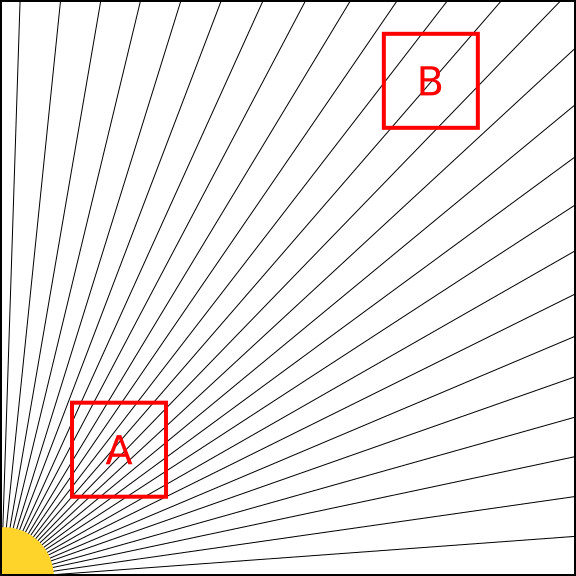
\includegraphics[width=\textwidth]{plots/CH2/rayDensityComparison.png}
    \caption{Ray density of a single source. Both regions A and B have the same area but region A intersects a far greater number of rays than region B.}
    \label{rayfig}
\end{figure}

One method used to mitigate this issue is to dynamically merge and split rays as they propagate so as to match the resolution of either the cells or the SPH particles such as is discussed in \citep{MORAYish} and implemented in MORAY \citep{moray}. This method utilizes a HEALPix sphere (see section \ref{sec:healpix}) of rays with equal solid angle where the number of rays at the source is fixed. As the rays interact with cells, they are checked against a refinement criterion where the number of rays intersecting the cell is logged. If there are too few rays, each ray is split into 4, with each child ray's direction set to give equal solid angles for all children. Likewise, if there are too many rays, the rays are collapsed into a single ray whose direction is the averaged direction of all child rays. This causes the number of rays sampling each cell to remain within set bounds and allows for a far more even sampling rate across the entire simulation box. Monte-Carlo methods that use rays for radiation propagation can also use this technique. 

While ray tracing is an excellent fit when looking to study the entire geometry of the system, it may not be the best method when looking to model scattering or if the distance individual rays travel is low. In this case, it may be preferred to use a simpler method such as FLD or to combine FLD with ray tracing algorithms.     

\section{Parallel codes and motivation}

Due to the high computational cost of radiative transfer, we need a large amount of computational power to run simulations with a high enough resolution to be realistic. This requires the use of High Performance Computing (HPC), where we utilize either very high clock rate single core processors or a combination of many processors into a multi-core system.

\subsection{The Limitations of Single Core Processors}

The two key methods to reduce computational cost without sacrificing resolution are the use of a processor with a greater clock speed or the use of multiple processors in unison. Single core processor speeds are closely linked to the size of their transistors which have historically reduced by a factor of two approximately every 18 months (a trend commonly known as Moore's Law). 

As the transistor gates decrease in size, electrons are more likely to quantum tunnel through the transistor gate, rendering them ineffective as transistors must reliably block the flow of electrons when closed. This places a limit on how small classical transistors can be manufactured before quantum effects begin to dominate.

The long running trend of the power usage remaining steady, regardless of the number of transistors, was also broken in the early 2000s due to the higher rate of thermal leakage in smaller transistors. The power draw is now approximately proportional to the cube of the transistor count, thus drastically increasing as we further reduce the transistor size. 

These issues, combined with the limitations on the amount of memory accessible to single core processors, makes it a challenge to scale simulations to high resolutions. This has led to the current standard of using multi-core systems.

\subsection{High Performance Computing}

The solution to the issue of high power usage in single cores has been to move from increasing the number of transistors to creating multiple cores on one chip. 2 cores running at half speed draw approximately a quarter of the power of a single core running at full speed while providing the same rate of computation. In principle, this not only reduces the cost of powering the system but also also reduces the amount of waste heat created. As cooling is often one of the larger expenses for data centres, this has a substantial impact on running costs.

Unfortunately, creating software that can run on multiple cores comes with many challenges. To discuss these, we will look at two types of parallel data management systems; shared data, where all cores have access to all data, and distributed data, where the data is distributed among multiple cores and each core only has access to its ``local" data.

With shared data, all cores are able to easily access any data they need and there is no need to synchronize each core but problems arise when multiple cores need to modify the same variable. As an example, say you have a function that adds to a shared integer. If a core attempts to access the integer while another is modifying its value, the core will fail to take into account the other core's contribution and thus return an incorrect value. Such issues are referred to as race conditions and require careful planning to avoid. This method also suffers from scaling limitations as the cores need to be within close physical proximity to the data storage medium to reduce latency.

Distributed data, on the other hand, stores a portion of the data set locally and in general is designed to only act directly on these data (e.g. with a gravity simulation, each core would calculate the gravitational force acting on each of their particles). This removes the possibility of a race condition for reads and writes as only one core is writing to any piece of data. It is still possible to create other similar issues but that is up to the programmer. Unfortunately, distributing data in such a way requires a far larger overhead as non-local data must be collected from other cores via message passing. The amount of data being stored on each core must be balanced with the rate and latency of data requests to ensure that the run time isn't dominated by message passing. The key benefit of distributed data is that the data is no longer bound to one storage device, allowing for the computation to be performed in multiple locations, possibly even multiple countries. This allows for access to far more memory and thus enables big problems to be tackled. For systems where latency isn't an issue, this can be used to take advantage of the vast computational power of consumer electronics, distributing computation to millions of personal computers and allowing for far greater data analysis than any one data centre could ever provide. An example of this is the BOINC software developed by the University of California \citep{boinc} where people can join programs to analyze massive data sets for such things as climate science and astrophysics.

To most effectively take advantage of parallel processing, the software must distribute the work among the cores in a way that minimizes the amount of time where multiple cores are idling while waiting for others to complete their tasks. This is known as Load Balancing. Typically this is also tied to the distribution of data (and thus limited by memory constraints per node).

\section{Summary of Thesis}

In Chapter 2, we look at the TREVR method for radiative transfer along with other existing methods for reverse ray tracing. We briefly discuss GASOLINE, the code base where TREVR was first implemented and how tree codes can be utilized to decrease computational cost.

Chapter 3 covers the implementation and methodology of the radiative transfer code in ChaNGa, discussing the key components of the Charm++ system and giving a detailed summary of the algorithms used.

Chapter 4 is focused on testing and analysis of the code, looking at the scaling of the method and finding appropriate values for the refinement parameters. 

Chapter 5 identifies the issue of complex sources as one not satisfactorily resolved in the original implementation of TREVR. We look at methods for resolving this without causing substantial increases to the algorithms computational cost. % Introduction

%\lhead{\emph{TRevR and Reverse Ray Tracings}} 
\chapter{Radiative Transfer in GASOLINE}

\section{Reverse Ray Tracing}

Reverse ray tracing is a method similar to standard (or forward) ray tracing but instead of tracing rays from each source through the simulation we instead trace rays from the sink outwards into the system, interacting with sources. This allows us to only trace rays where required, avoiding the issue shown in figure \ref{rayfig}. This also has the benefit of allowing us to take advantage of the tree structure by merging distant sources together into a single source, substantially reducing the computational cost. 

Probably the most important advantage is that we only perform the source walk for active sink particles. This way we can use adaptive time stepping and the amount of radiation work scales linearly with the size of the active subset, just as for gravity and hydrodynamics. Thus, we retain the advantages of adaptive time stepping, giving a wall-clock speed-up of order 100 times for gravity and hydro.

Reverse ray tracing doesn't suffer the issue of over or under-sampling of rays based on the position of a source in the system seen in forward ray tracing due each sink tracing a set number of rays from itself, with the quantity being either predetermined or based on refinement criterion. Thus there are no Monte Carlo errors in the flux associated with forward ray tracing. Further optimization such as ignoring sources with minimal flux contribution can also be utilized, something that is impossible to do with forward ray tracing codes due to not knowing the full list of sources a sink interacts with until the full ray trace has been completed.

Other minor advantages include knowing the distance to the sink when we walk. This allows us to use the light travel time to take into account the correct age of the source and apply red-shift corrections or spectral changes due to absorption.

\section{Existing Reverse Raytracing codes}

\subsection{TreeCol}
\label{sec:healpix}
TreeCol \citep{treecol} utilizes reverse ray tracing to produce a spherical column density map of the system for each sink particle  through information stored in the gravity tree. This is calculated during the gravity walk, minimizing the amount of communication required between sections of the tree stored on different CPUs. Originally implemented in the GADGET code \citep{gadget}, it uses an oct-tree as the basis for its tree walk.

The HEALPix algorithm is used to calculate the starting directions of the rays. HEALPix is a method for partitioning a sphere into ``pixels" of equal area \citep{healpix}. Utilizing such pixels guarantees that the sky around each sink is fully and equally sampled as all rays will subtend a roughly equal solid angle in the sky. Additionally, increasing the pixel number increases the angular resolution everywhere on the sphere by an equal amount. Latitude-longitude discretisation methods suffer from higher angular resolution of pixels at the poles and thus do not gain this benefit.

Each ray is traced from the sink to the edge of the system. At each node that passes the refinement criterion, the absorption properties are ``smeared" across the node and the node's contribution to absorption is calculated. For nodes whose bounds are only partially intersected by the cell, only the fraction of the cell that intersects contributes. Particle level refinement is performed by projecting the SPH particles as squares in the sky who's side lengths $r_n$ are calculated to give an area equal to that of a circle of radius equal to the smoothing length $h$ such that,
\begin{equation}
    r_n = \frac{1}{2} \sqrt{\pi}h.
\end{equation}
A square profile is selected over the standard circular one due to the computational complexity of calculating the ``true" fraction of the SPH particle that intersects with the HEALPix pixel as the pixel and particle have quite differing shapes. This would require numerical integration over the overlapping areas and would still only give an approximate value.

\subsection{URCHIN}

URCHIN \citep{urchin} is a reverse ray tracing scheme designed to model self-shielding from post-reionization UV background radiation in cosmological simulations. Instead of utilizing a binary tree, URCHIN traces a fixed number of rays (by default 12) from each sink and interacts directly with the resolution elements (be it SPH, mesh, etc) that the ray intersects. The direction of each ray is once again selected through the use of a HEALPix sphere and no refinement process is applied. Instead optimization is gained by treating all particles outside self-shielded and proximity zones as correct in the uniform, optically thin limit. Reverse ray tracing was selected over forward ray tracing due to the greater accuracy when modelling background sources, uniform sampling of sources and the ability to sample a broad range of spectral bands.

To begin, the neutral fraction of each particle is set to its optically thick value, allowing for the H1 column density to be calculated along each ray. The shielded photoionization rate is then calculated (see \citealt{urchin}) along with an effective optical depth. Resolution elements whose effective optical depths are below a set threshold are treated as optically thin for subsequent iterations. All other elements are iterated over until the change in neutral fraction is within acceptable bounds and thus the elements are treated as converged. For typical values, this convergence occurs within 5 iterations for 99\% of elements.

\subsection{TreeRay}

TreeRay \citep{treeRay} was developed for the FLASH AMR code \citep{flash} to model ionizing radiation from massive stars. TreeRay takes advantage of the preexisting gravity oct-tree in FLASH, once again tracing a multitude of rays around each sink who's directions are calculated using a HEALPix sphere. Each ray is split into multiple segments with lengths increasing linearly as you move away from the target cell. This causes the segment lengths to approximately correspond to the physical size of the nodes that pass refinement.

During the tree traversal, the contribution of each node to the ray segments is calculated by mapping the densities, radiation luminosities and energy fluxes according to the amount that the ray intersects the node volume. Once the walk is complete, the 1D radiative transport equation is solved along each ray, along with physical properties such as the Str{\"o}mgren radius and the recombination rate (see \citep{treeRay}). By drawing a fixed number of rays from each source, the computational cost of this algorithm is independent of the number of sources, allowing for the simulation of radiative feedback of many stars.

\section{GASOLINE}

GASOLINE \citep{gasoline} is an N-body Smoothed Particle Hydrodynamics (SPH) code developed to simulate astrophysical hydrodynamics with self-gravity Separate trees are built for all components of the system (e.g. gravity, SPH, radiation), allowing for data from previous components (such as density from SPH) to be used in the first tree builds but adding to the overhead of each step. When GASOLINE was developed, the ratio of time spent running computation to time spent building the tree to was more than 100:1, making the added computational cost of multiple tree builds negligible \citep{rory}. This is no longer true with adaptive timestepping for the dynamical ranges achieved currently and motivated design changes for ChaNGa as discussed in Chapter \ref{sec:ChaNGa}.

As GASOLINE is built upon PKDGrav \citep{pkdgrav}, a N-body gravity code, SPH was the most applicable method for hydrodynamics. Refer to \citet{wadsley2017} for a current description of the physical models, algorithms and code performance on tests. 

\subsection{Tree Codes}

Originally outlined in \cite{gravity}, data trees can be utilized to drastically reduce the computational cost of calculating gravitational forces. Existing N-Body methods at the time mainly relied on directly calculating the force between every particle pair, resulting in a cost of $\mathcal{O}(N^2)$ where N is the baryon count of the system. By splitting the simulation volume into a tree of nested boxes, or nodes, each containing combined physical properties such as the total and centre of mass of their children, we can treat entire nodes as single sources. This process is repeated until either only one particle remains in the node or in some cases until under a set number of particles remain.

Unfortunately, nodes higher in the tree act as a poorer estimate of the true particle properties and thus create larger errors in the gravitational force. Because of this we require a criterion for deciding if a node should be opened. The method developed by Barnes and Hut was to take the maximum dimension of the node being considered and divide it by the distance between that node's centre of mass and the particle being walked. If this value is greater than a chosen ``opening angle", the angular size of the node in the sky as seen by the particle is too great and the node is refined. Otherwise, the node is considered to be an accurate representation of the constituent particles and can be used to calculate their contribution to the gravitational force. This substantially reduces the number of calculations required, giving a cost of $\mathcal{O}(N \log(N))$ where N is the number of particles (assumed to be proportional to the number of tree nodes. 

One method utilized by Barnes and Hut to reduce the error caused by the opening angle is to implement a multipole expansion. In their case, they used a quadrupole expansion causing the first error term to be $\mathcal{O}(dx^3)$ where $dx$ is the physical size of the node being expanded. Higher order expansions give smaller error terms and thus allow for a larger opening angle to be used while retaining a given error. GASOLINE utilizes a hexadecapole expansion for gravity, giving it a leading error term of $\mathcal{O}(dx^5)$. this gives better than 1\% errors for an opening angle of 0.7. TREVR, on the other hand, is monopole, giving a leading error term of $\mathcal{O}(dx^2)$, requiring a smaller opening angle for the same error.

There are several ways that the simulation volume can be split. The first is with an oct-tree, where each node is split into 8 equally sized sub-nodes by equally bisecting the node in all three dimensions. Alternatively, one can bisect in only one dimension at each level creating a k-d tree. Equally bisecting at each level effectively simulates an oct-tree every 3 levels.

\section{The TREVR Radiative Transfer Method}

Designed and implemented in the GASOLINE SPH code by Rory Woods, James Wadsley and Hugh Couchman \citep{rory} and expanded upon by Jasper Grond \citep{grond}, TREVR (Tree-based REVerse Raytrace) is an adaptive radiative transfer scheme that can be applied to both SPH and grid-based codes. By walking from the sink to the source we utilize a tree similar to the gravitational force computation, combining distant sources to reduce computational cost. In TREVR, we trace exactly one ray between each sink-source pair, where the source can be either an individual star particle or a combined source node. This gives a computational cost for the optically thin regime of $\mathcal{O}(N_{sink}Log(N_{source}))$.

To calculate optical depths TREVR utilizes a tree, combining absorbers where the loss in accuracy is within acceptable bounds as described in section \ref{sec:sourceRef}. TREVR uses a similar method for the optically thick walk, combining nodes whose absorption properties give a good approximation of their component absorbing particles. This is described in detail in section \ref{sec:thickRefine}. The optical depth of the ray is computed at each step in the walk by calculating the length of the ray segment passing through the node's bounding box which is combined with its averaged absorption properties.

While the utilization of a tree makes this algorithm suitable for a grid code, some form of SPH-like approach must be implemented for the ``last mile", where refinement to the individual absorbing particles is required. Failure to do this can cause incorrect results for such things as the propagation of ionization fronts. This was convenient when developing TREVR as the existing SPH code could be utilized for the particle level ray tracing. TREVR controls refinement in the radiation code by utilizing an opening angle criterion while searching for sources (see section \ref{sec:sourceRef}) and refines based on the maximum optical depth variation of the node for the optically thick walk (see section \ref{sec:thickRefine}).  % Radiative Transfer Methods

%\lhead{\emph{Implementation}} 
\chapter{TREVR Implementation In ChaNGa}
\label{sec:ChaNGa}
In this section we will give an overview of the Charm++ framework as well as the ChaNGa code that is built upon an extended version of the Charm++ framework. We discuss the methods used to develop the radiative transfer code and some of the challenges faced during implementation.

\section{Charm++}
Charm++ is a framework built upon the C++ language designed for applications in MIMD (Multiple Instruction, Multiple Data) parallel codes. Charm++ was designed to significantly reduce the quantity of coding work required when attempting to run parallel codes on multiple computer systems. This usually requires bespoke codes for every system in order to take into account memory type (i.e shared or distributed), message passing method and other system specific details \citep{Charm1}. This resulted in a large amount of developer time being spent on machine specific code rather than science related code. Through the use of the Chare class and object described in section \ref{sec:chare}, these issues are resolved via a runtime support system, hidden from the developer \citep{Charm2}.

Charm++ has several goals in its design: portability, where the same code can be run on all MIMD systems without modification; dynamic load balancing, where irregular parallel computations are handled so as to reduce core idle time; and latency tolerance, where requests for remote data do not force the core to idle while local work can still be performed \citep{Charm1}. Dynamic load balancing is performed through the use of Chare objects and latency tolerance through the use of a non-blocking message passing system. These are discussed in detail below.

Charm++ has been shown to scale excellently with large numbers of cores, as shown by the NAMD molecular dynamics code that showed speedup of 1599 times single core speeds when running on 2250 cores \citep{NAMD} although this simulation did not use the chare class, instead opting for custom Charm++ code. As molecular dynamics only has of order 100,000 computational elements (e.g. atoms in a protein), being able to divide work efficiently is a major achievement.

\subsection{The Chare Class}
\label{sec:chare}
The core component of a Charm++ program is the Chare class. The following outline of Charm++ and chares follows \citet{Charm2} and the Charm++ manual. Chares are concurrent objects that contain private data and a series of entry points, acting as the functions for the class. Each entry point takes a single input, a pointer to a message containing all data relevant to that function, and has no return value. As the Chare class is designed to avoid blocking remote access, it cannot contain public members. Chares can be distributed among all available cores and each core can hold multiple Chares. At any one time, a serial core only runs one Chare and that Chare only runs one entry function. This means that so long as the entry functions are written in such a way that they only modify local data, it is unlikely that race conditions will occur. Each Chare is given a handle unique across all processors that acts as its identifier for message passing which is handled by the run-time system for Charm++ rather than explicitly by the user.

A subclass of Chares, known as Branched Chares, have a branch on all processors. These are identified by a unique handler and share a similar definition syntax to standard Chares, with the addition of ``branched" at the start of their type definition. Once a Branched Chare has been created, usually by the main Chare, it is possible to call an entry function on all branches of that Chare simultaneously, allowing for simple control of all processes from a single command. Similarly, entry functions can be ran on an individual Chare by either calling them from within the Chare itself or by referencing its handle.

For every Charm++ program, there must be exactly one instance of the Chare type ``Main", executed on a single core. This begins the execution process and is often used to initialize shared variables and create new Chares. 

\subsection{Message Passing}

Message objects are utilized in Charm++ to allow for effective communication between chares and function scheduling while increasing code visibility to developers, aiding understanding and reducing complexity. These messages encapsulate all of the parameters to be sent to an entry method and thus different entry method calls can require different message types that can be created to hold any required data. This allows for developers to transfer data, including complex data structures, between chares without having to interact directly with message passing code.

Messages are stored when received by a core, requiring explicit deletion. This creates the risk of memory leaks as a result of poor programming practices but allows for messages to be acted upon in any order once received. When a message is created the programmer assigns a priority where lower values denote higher priorities by default. This is of particular use during tree walks as it allows us to prioritize messages returning data from remote walk data requests over local walk function calls, ensuring that the data is acted upon as received and freeing the memory required to store the message for further use. If multiple received messages have identical priority, they are computed in first-in-first-out order. 

\section{ChaNGa}
\label{sec:ChaNGa}
ChaNGa (CHArm N-body GrAvity solver) is an N-Body SPH and gravity solver adapted from GASOLINE. It was developed by the N-Body Shop research group at the University of Washington in collaboration with the University of Illinois Parallel Programming Laboratory to overcome the scaling issues encountered by GASOLINE on more modern machines whose processor counts are in the thousands \citep{ChaNGa1}. It is designed as an extension of the University of Illinois Charm++ framework. Specific extensions to basic Charm++ for ChaNGa include load balancing for adaptive timestepping. The core scientific modules are directly comparable to those of GASOLINE, with near identical methodology for SPH and cooling.

Like GASOLINE, ChaNGa uses a binary tree to split the simulation space but ChaNGa always splits cells in X-Y-Z order, effectively replicating an oct-tree every 3 levels. This allows Oct-tree-based methods for work distribution to be utilized \citep{ChaNGa1}. The tree is split into ``tree pieces", Chare objects (see section \ref{sec:chare}) that are distributed among the cores in use. By default there are 8 tree pieces created per core, each with a subset of the full tree. Each typically includes all the parent node information as well as all particles inside all nodes owned by the treepiece. All other particles must be requested as cached copies of the originals that are owned by other tree pieces. These other tree pieces can be both local (i.e. stored on the same processor) or remote (stored on another processor). 
\\
\\
\\
ChaNGa, again like GASOLINE, is designed to utilize adaptive time-stepping that allows for high time resolution in regions with short dynamic timescales without causing a substantial increase in wall time due to having to compute all particles at this timescale. Performance evaluations have shown up to 3x speedup over single stepping algorithms on NCSA's Blue Waters system \citep{ChaNGa3}

ChaNGa includes a system for ``checkpointing" where the entire state of the system is dumped to file. These checkpoints allow for the code to be restarted in cases such as hardware failure while ensuring no change to the output of the system. This is of particular importance when the data is highly sensitive to small changes in the system state, such as is the case in astrophysical simulations.

While regular checkpointing is recommended, the high cost of writing such a large quantity of data to storage requires a balance to be found between the possible data recovery gains and the cost in time.
    
\subsection{Space Filling Curves}

GASOLINE was developed to distribute data by splitting the data into a balanced binary tree, assigning the data on each leaf node to a core. This often led to the tree being split into long, thin slices and required a large amount of overhead, particularly when using more than 8 cores. This limited the scaling of GASOLINE, suggesting a need for a new method when developing ChaNGa.

For algorithms such as neighbour finding in particle methods or particle tracing in radiation (see section \ref{sec:ppWalk}), where the input data is in close physical proximity to the datum being computed, the data can be sorted, in theory decreasing the amount of overhead. This can be done by mapping the positions of the data to a space filling curve, a function that is continuous in space and can be iteratively refined so as to match the resolution of the data. This results in a large portion of the computation for each node using local data, with only the boundary data requiring requests to be sent to remote nodes.


While ChaNGa was initially built to use the Morton space filling curve (SFC), it was later adapted to use the Peano-Hilbert SFC. This curve is theoretically more efficient due to the lack of the Morton curve's sharp jumps. This increases data locality, where particles with close physical proximity also have close key proximity. This is an advantage in most serial and parallel computation. This also adds to the complexity of the code when calculating the physical bounds of the particles assigned to each node. Unlike the Morton SFC the Peano-Hilbert SFC rotates the shape used to create its curve, creating a disconnect between the spatially defined children and the ordering of the child nodes given by the SFC. For example, this removes the guarantee that child 0 of the node is assigned the particles who's indices are numerically lower than those of child 1, as shown in figure \ref{fig:SFC}. In this figure, the green regions show the cells with lower key values while the yellow shows that of higher key values. The Morton SFC's left hand child, equivalent to child 0, always contains the lower set of keys, unlike the Peano-Hilbert SFC. Because of this, the Morton SFC was utilized when running with the radiation code over the Peano-Hilbert SFC that is the default for ChaNGa.

\begin{figure}[H]
    \centering
    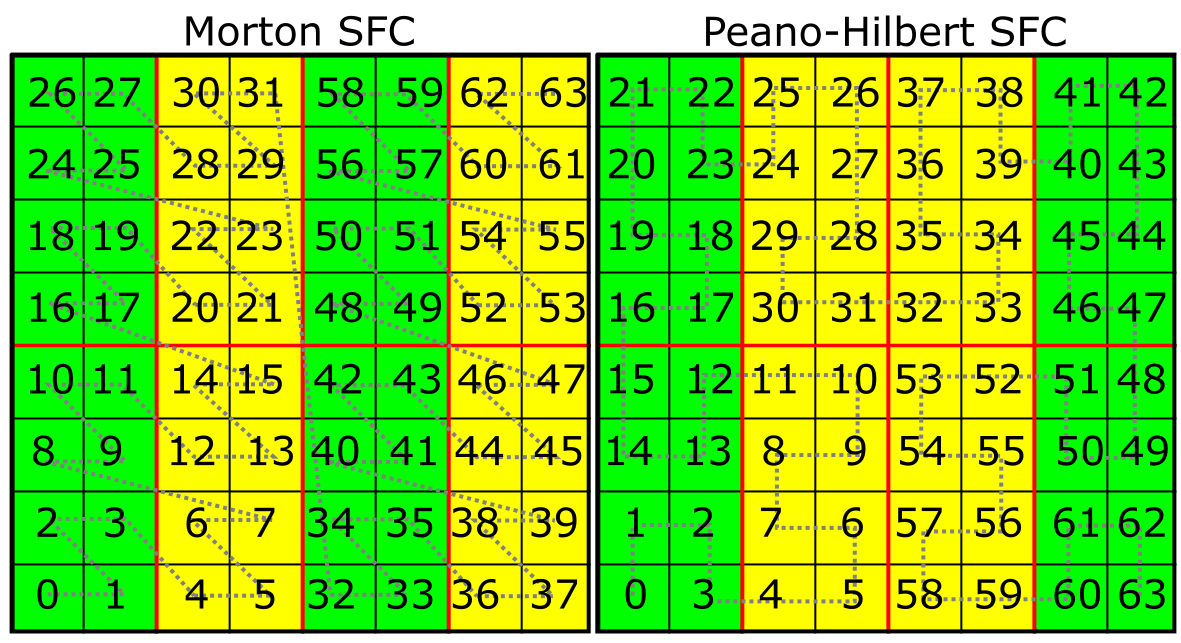
\includegraphics[width=\textwidth]{plots/CH3/SFCCompare.png}
    \caption{Diagram of Morton and Peano Hilbert space filling curves after 3 bisections (in the x, y and x axis respectively) 64}
    \label{fig:SFC}
\end{figure}

When the Morton SFC was replaced with the Peano-Hilbert SFC the bounds defining the node volume no longer consistently contained the particles assigned to the node. As a part of the tree build, the bounds are recalculated so that they define the minimum volume that contains all particles in the node (for identical reasons to those discussed for sources in section \ref{sec:sourceRef}). This bug remained undetected until the development of the radiation code as no other component of the code requires the exact spatial dimensions of each node and thus suffered no errors as a result of this. 

\subsection{The Tree Build}

To begin, the particles are assigned a key based on their position using a space filling curve (SFC). This curve is a fractal that can be refined as required to match the resolution of the particles in the system. These keys are then used during the tree build, where the particle set is bisected along each axis in turn to create child nodes. By bisecting at the key value associated with the bisection point in the space filling curve, we can accurately allocate the particles without having to check their individual positions, reducing the computational cost. This process is repeated for each node until the number of particles in the child node is lower than a predefined value. These final nodes are labelled bucket nodes and for ChaNGa the cutoff particle count is 12 although this can be changed by modifying the ``nBucket" parameter specified in the input parameter file for a given run.

Once the bucket nodes have been created the process is reversed, now walking from the bucket to the root. First, the node properties such as centre of luminosity and total luminosity are calculated for all buckets and then these values are propagated up into the parent nodes. This is repeated until all nodes have their properties calculated from their child nodes resulting in a tree that can be walked from both top down and bottom up depending on what is required.

While a new tree is built for every physics solver of GASOLINE, ChaNGa only builds the tree once per timestep, before any physical quantities (e.g. density or forces) are estimated, and uses it for every part of that timestep. Early in the development of GASOLINE the tree build was only a small fraction of the computational cost. The addition of adaptive timesteps has greatly impacted this as a tree must be built for each physics solver even if only a few particles are active, resulting in a large percentage of the time being spent building trees. 

While only building the tree once reduces overhead, it lacks the flexibility of GASOLINE's method where variables calculated in previous sections of the code can be easily included in the tree. For ChaNGa, an additional tree build is required once the required variables, such as density which is calculated as a part of the SPH code, have been calculated. This is a key issue for radiation due to the importance of density in the absorption coefficient. Values from prior time-steps could be used, either directly or through extrapolation.

A key benefit of the combined tree build is the simplicity it adds to the development of new code components. While implementing the radiation code, all that was required to propagate the radiation properties through the tree once they had been defined was two function calls: one for adding a new particle to a bucket and another for combining two child nodes into the parent node. These could be stored alongside the rest of the radiation code, minimizing the amount of code bloat that can arise from multiple new components being added to the original tree build. It also means that any modifications to the tree build will have little impact on the radiation properties so long as the function calls remain in the correct locations.

\subsection{Issues when developing on ChaNGa}

Unfortunately, development on ChaNGa suffers from several issues. The documentation lacks details on the specifics of developing the code other than for minor changes such as the addition of new parameters. This leaves those working on the more detailed sections of the code such as the tree build and data management systems reliant on comments in the code itself. These comments are often non-existent or insufficient and much time was required to properly understand their function. This combined with poor adherence to a standard formatting style leads to a difficult development process. Much of the code has substantial variation in indenting styles (or no indentation at all), comment format and variable name styles. Recently, efforts have been made to define a standard style for all collaborators to adhere to. Special thanks must be given to Tom Quinn from the University of Washington for the substantial amount of support and advice when developing the radiative transfer code, without whom many of the issues encountered would have taken far longer to resolve.

\section{TREVR in ChaNGa}

Although the core concepts behind the implementation of TREVR in ChaNGa are identical to those in GASOLINE, there are some key differences in the structure and methodology of the two codes that required new approaches to be developed.

\subsection{Top Down vs Bottom Up Tree Walk}

During the development of the radiation code for Gasoline, it was decided that the preferred method for the tree walk was a Bottom-Up approach, where the tree walk starts at the leaf node of the particle being walked from and moves up the tree till it reaches the root node. A second walk could then begin from the leaf node containing the source particle to the root, terminating if it reaches a node also walked by the sink.

Discussions with the developer Rory Woods revealed that this decision was made due to how the walk would focus resolution at the areas around the sink and source, areas which are often of the most interest when performing the ray trace. When using a refinement criterion to decide if a cell should be opened, this no longer holds true and the bottom-up tree walk acts in a similar way to the top-down tree walk but generally walks more nodes than necessary. While in the initial version of TREVR the refinement was purely geometric, the newest version of TREVR (\citealt{grond}) uses an adaptivity criterion instead.

Due to the more complex dual-walk method required for the bottom-up tree walk, the top-down tree walk was selected for implementation in ChaNGa. This method walks to both the sink and source simultaneously, removing the need to check if the second walk has reached a shared node with the first walk. This also has the benefit that if the system passes the refinement criterion on a high level node (such as for sources with a single or tightly clustered sources, as discussed in the next section), the tree walk can be completed very rapidly. Unlike the GASOLINE method, this means that for low average optical depths the computational cost of the optically thick tree walk can be less than $\mathcal{O}(log(N))$.

\subsection{Developing the Source Walk}

To begin the radiative transfer process we set up the book-keeping variables that allow us to keep track of how many remote data requests have been sent out for each bucket as well as which buckets have had their local and remote walks completed. We then loop through all buckets, starting both the local and remote walk for each. To allow for remote messages to be acted upon, the loop is paused at a set number of buckets and the function re-queued in the scheduler. This allows for local work to be performed while waiting for the remote requests and reduces the time that each core spends idling.

During the walk each node is checked against the opening criterion (see section \ref{sec:sourceRef}) to see if it requires refinement. If no refinement is required, the properties calculated via upwards propagation from the bucket are used to calculate the contribution to the flux from the the combination of sources in that node. If the node must be refined further, either the children of that node are walked or, in the case of bucket nodes, the flux contribution from each component source is calculated. This is repeated until the flux contribution from the entire system is calculated.

While the flux on each particle in the bucket is calculated using the individual particle's position, we use the centre of mass of the bucket as the basis for the opening criterion and thus all particles in a bucket have the same sources. This reduces the number of walks required by a factor of up to the maximum number of particles per bucket while adding minimal error.

\subsection{Source Walk Refinement criterion}
\label{sec:sourceRef}
Like the gravity code, the radiation code uses an opening angle based refinement criterion. The maximum distance from the centre of luminosity to the edge of the cell, $b_{max}$, along with the minimum distance between the sink and the physical boundary of the cell, $r$, are used to limit its angular diameter, giving,
\begin{equation}
    \label{eqn:openingTheta}
    \theta = \frac{b_{max}}{r}.
\end{equation}
A node is opened when the value of $\theta$ exceeds a predefined opening angle $\theta_{open}$.

As combining sources affects the accuracy of the calculated flux due to changes in the value of $r$, a balance must be found between computational savings and accuracy. To do this, the number of nodes walked, a good indicator of computational cost, can be calculated for multiple opening angles and the results compared to those for a fully opened version of the same system. This is explored further in section \ref{sec:bangForBuck}.

ChaNGa includes a collection of geometric intersection algorithms and it is thus easier to write equation \ref{eqn:opening} in terms of $r_{open}$, where $r_{open}$ is the radius of a sphere centred on the sink. If the rectangle defining the volume contained by a node intersects with this sphere, that node must be refined,
\begin{equation}
    \label{eqn:opening}
    r_{open} = \frac{b_{max}}{\theta_{open}}.
\end{equation}
The refinement criterion test can now be performed by creating a sphere of radius of $r_{open}$ and using the intersection algorithms to check if the sphere intersects the bounding cell of a node, as shown in figure \ref{fig:opening}.

\begin{figure}[H]
    \centering
    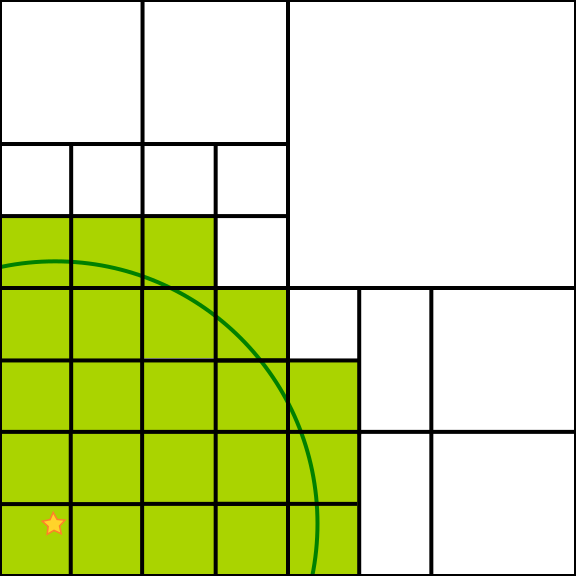
\includegraphics[width=0.9\textwidth]{plots/CH3/openingCritereon.png}
    \caption{Diagram of opening criterion for the source walk. All nodes that intersect the sphere of radius $r_{open}$, shown in green, are refined.}
    \label{fig:opening}
\end{figure}

Unlike gravity, where all particles inside a node contribute to its mass and thus must be considered, the only particles that contribute to the flux are sources, similar to how only SPH particles are considered during the fluid code. Because of this, a cell containing only the source locations can be considered when calculating the value of $b_{max}$. For a system with a single source, this means that the root node can accurately describe the entire system and thus the computational cost of the tree walk can be drastically reduced. In astrophysics, sources are often grouped together (star clusters, galaxies, etc) and thus this change should allow for less walking required in most applications. An example of this is shown in figure \ref{fig:sourceBoxes}.

\begin{figure}[H]
    \centering
    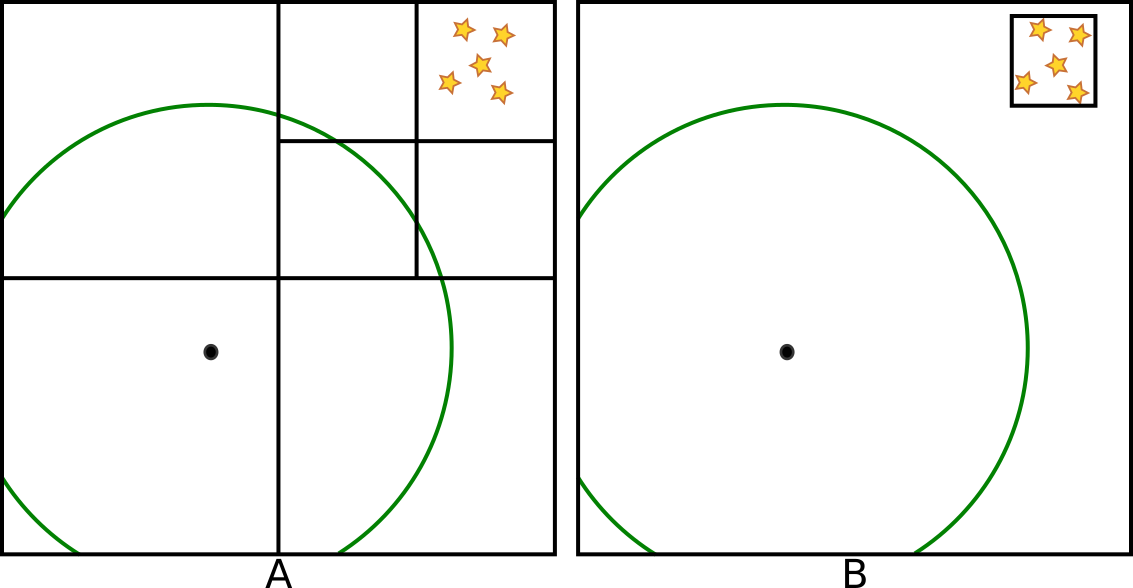
\includegraphics[width=\textwidth]{plots/CH3/sourceBox.png}
    \caption{Diagram of the effect of reducing the node's bounds so that they define the minimum volume that contains the node's source particles. A must refine to the 5th level in the tree whereas B can use the root node.}
    \label{fig:sourceBoxes}
\end{figure}

This is performed by utilizing code similar to that used for the pre-existing bounding boxes used for gravitational forces that are bounded by the particle positions in the node. To build a bounding box only containing the sources, first an empty box with zero volume is created and each source in the node is added through the use of the ``grow" function in the OrientedBox class used to define the node bounds. This updates the limits of the bounding box so that they contain all source particles in the node in the smallest possible volume.

\section{The Optically Thick Tree Walk}

\subsection{Developing the Optically Thick Tree Walk}

Instead of immediately calculating the flux contribution once a source has been located we store the source's position and total luminosity in an array for later use. As the source walk is run on the bucket rather than per particle, we only require one list of sources for all particles in a single bucket, reducing data usage. This results in a complete list of all sources for all sinks in the system once the source walk is complete. While this requires a large amount of data to be stored it has the benefit of allowing us to estimate the total flux on a sink before starting the optically thick walk. The uses of this are discussed in section \ref{sec:complexsources}.

The particles are walked one source at a time, with all sources for all particles in a bucket run before the next bucket is started. At the start of the walk, the optically thin flux is calculated for the sink-source pair being walked and stored in a placeholder variable on the sink. Once a walk is completed the sink particle being walked checks if any sources remain and if so begins the next walk.

During the walk, each node is checked for refinement, where nodes whose averaged absorption parameters are a poor estimate for the true optical depth through the node are refined (see section \ref{sec:thickRefine}). Once a node is selected, the length of the ray segment through that node and the node's absorption parameters are used to calculate the contribution to the optical depth. Once the full ray has been traced, the calculated optical depth is combined with the previously calculated optically thin flux to give the final flux via equation \ref{eqn:fluxThick}

\subsection{Calculating Optical Depths}
During the tree build, each bucket in the tree has all of its radiation properties calculated from its component particles. For the absorption coefficient, this was done originally through the method of summing each particle's product of mass and opacity and dividing by the total cell volume as shown in equation \ref{eqn:calcAbsCoeff} \citep{rory},
\begin{equation}
    \alpha_{bucket} = \frac{1}{N_{abs}}\sum_i{\frac{\kappa_i m_i}{V_{bucket}}},
    \label{eqn:calcAbsCoeff}
\end{equation}
where $V_{bucket}$ is the volume of the bucket, $N_{abs}$ is the number of absorbers in the bucket and $\kappa_i$ and $m_i$ are the absorber's opacities and masses respectively.

Unfortunately, this is susceptible to noise due to variations in particle counts per cell, especially if the number of particles in the cell is low . Solutions to this issue involve using a smoothed density estimate such as that estimated on each particle for SPH. These can then be averaged within a bucket. 

This creates a second issue where, because SPH, gravity and radiation are computed at the same time, up-to-date density estimates are unavailable during the tree build. Solutions to this second issue include using densities from previous timesteps, rebuilding the tree once density has been calculated, and extrapolating densities using known values. One such extrapolation method is to use the previous timestep's densities and the divergence of the particle velocities to give,
\begin{equation}
    \rho_i = \rho_{i-1} + \frac{d\rho}{dt}dt = \rho_{i-1} + \rho_{i-1} (-\bm{\bigtriangledown \cdot v} dt),
\end{equation}
where $\rho_i$ and $\rho_{i-1}$ are the current and previous timestep's densities respectively \citep{divV}.

Once the absorption coefficient for every bucket is calculated, the rest of the tree's absorption coefficients can be calculated by averaging those of each node's children.

During the tree walk, each node is checked to see if it intersects with the ray between the sink and the source and if so, the length of the segment contained within the node is computed. The node is then checked for refinement and if necessary the optical depth contribution for that node is calculated using the discrete form of equation \ref{eqn:tau}, shown below,
\begin{equation}
    \tau_{node} = \alpha_{node} s_{int},
\end{equation}

where $\alpha_{node}$ is the node's absorption coefficient (which includes the opacity term) and $s_{int}$ is the distance of the intersecting segment of the ray.

\subsection{Ray Trace Walk Refinement Criterion}
\label{sec:thickRefine}

As with the source walk, we need a method of deciding if a tree node is suitable for ray tracing or if it must be further refined. Just as the source walk's accuracy is decreased as sources are merged, the ray trace walk's accuracy is decreased when the absorption coefficients are taken from merged tree nodes.

Simply looking at the coefficients of the two children nodes is insufficient due to the ``smoothing" of the absorption coefficient as one moves up the tree. To resolve this issue, we instead create a best and worst case path through each node in all 3 dimensions. The best case path is set of buckets that gives the lowest optical depth through the node. For example, if looking for the best case path in the x direction, it would be the collection of buckets with the lowest absorption coefficients where no two buckets share the same position in the x axis. The positions in the y and z axis are unconstrained so that the buckets may not be continuous in space.

When two buckets are combined, the parent node stores the the greatest absorption coefficient or the averaged absorption coefficients of each child for each dimension depending on which dimension is being merged. (E.g. when merging two cells split along the x axis, the maximum in the x direction is the average of the two bucket's maximum absorption coefficients and the maxima for the other two directions are the greatest of the two absorption coefficients. Likewise for the minimum). This is then repeated on higher level nodes, with either the maximum/minimum or average of the maxima/minima absorption coefficients propagated, resulting in two values that represent the paths through the node with the thinnest and thickest optical depths. This path does not have to be physically possible for a ray to cross (i.e. the nodes used to create it do not have to be continuous in space) but it still provides as an effective bound for the theoretical error in each node. We must also take into account the length of the segment intersecting the node being walked. This prevents excessive refinement in the case of a small segment passing through a region with high variance in its absorption coefficient. While the percentage error for that segment may be large, the segment's overall contribution to the ray remains small enough that the total error is limited. This also allows us to use a single value for the opening criterion that will work for the entire ray trace.

To perform the refinement test, the difference in minimum and maximum absorption coefficient for all cardinal directions is multiplied by the segment length to give a theoretical maximum error in $\tau$, as shown in equation \ref{eqn:thickRefinement},
\begin{equation}
    \delta\tau = l_{seg}(\alpha_{max} - \alpha_{min}),
    \label{eqn:thickRefinement}
\end{equation}
where $\delta\tau$ is the error in $\tau$, $l_{seg}$ is the segment length and $\alpha_{min}$ and $\alpha_{max}$ are the minimum and maximum $\tau_{refine}$ through the node. If $\epsilon_\tau$ exceeds the refinement parameter the node is opened and the children walked. To avoid self absorption, we also refine all nodes whose bounds lie or partially lie within the smoothing length of the sink being walked. This refinement creates an approximation of a sphere inside which the ray tracing moves from particle-node absorption to particle-particle absorption.

\subsection{Particle Level Ray Tracing}
\label{sec:ppWalk}
While node-level calculations of the optical depth are simple, only requiring the appropriate node to be selected via the opening criterion, refinement to the particle level requires more consideration. To correctly resolve ionization fronts (such as those seen in Str{\"o}mgren sphere tests) the ray must be traced through all particles in close proximity to the sink being analyzed. This prevents the sharp jump in opacity at the ionization front from being smoothed out by the averaging of properties during the tree build. This portion of the computation is referred to as Particle-Particle (PP) absorption. The method used for this was adapted from that used in the GASOLINE implementation of this code \citep{rory}.

To begin, the gas particles needs to be converted into a form that can be ray traced. To do this, we flatten the particle into a 2d disk in the plane perpendicular to the ray, with radius equal to its smoothing length, h (as calculated in the SPH code). We then need to calculate the minimum distance between the ray and the absorbing particle's position. As the ray is defined by the line between the sink position and source position, this distance can be calculated using the following equation,
\begin{equation}
d = \sqrt{||\bm{x}_0 - \bm{x}_2||^2 - \frac{((\bm{x}_0 - \bm{x}_2) \cdot (\bm{x}_1 - \bm{x}_2))^2} {||\bm{x}_1 - \bm{x}_2||^2}},
\end{equation}
where ${\bm{x}_0}$ is the particle location and ${\bm{x}_1}$ and ${\bm{x}_2}$ are the sink and source particle locations respectively.

Once we have this distance, we can calculate the optical depth contribution by passing the distance and smoothing length of the particle to an integrated smoothing kernel, giving us a contribution to $\tau$ of,
\begin{equation}
\tau_i = \kappa_i m_i \int{W \bigg(\frac{d_i}{h_i}\bigg)}ds,
\end{equation}
where $\kappa_i$, $m_i$ and $h_i$ are the absorber's opacity, mass and SPH smoothing length, $W(x)$ is the SPH smoothing kernel function and $ds$ is the segment of the ray intersecting the absorbing particle.

This smoothing kernel, shown in figure \ref{smoothingKernel}, represents the radial distribution of the absorbing mass over a sphere whose radius is equal to twice the smoothing length. Integrating this gives the effective density of a path through the sphere perpendicular to the radial direction. 
\begin{figure}[H]
    \centering
    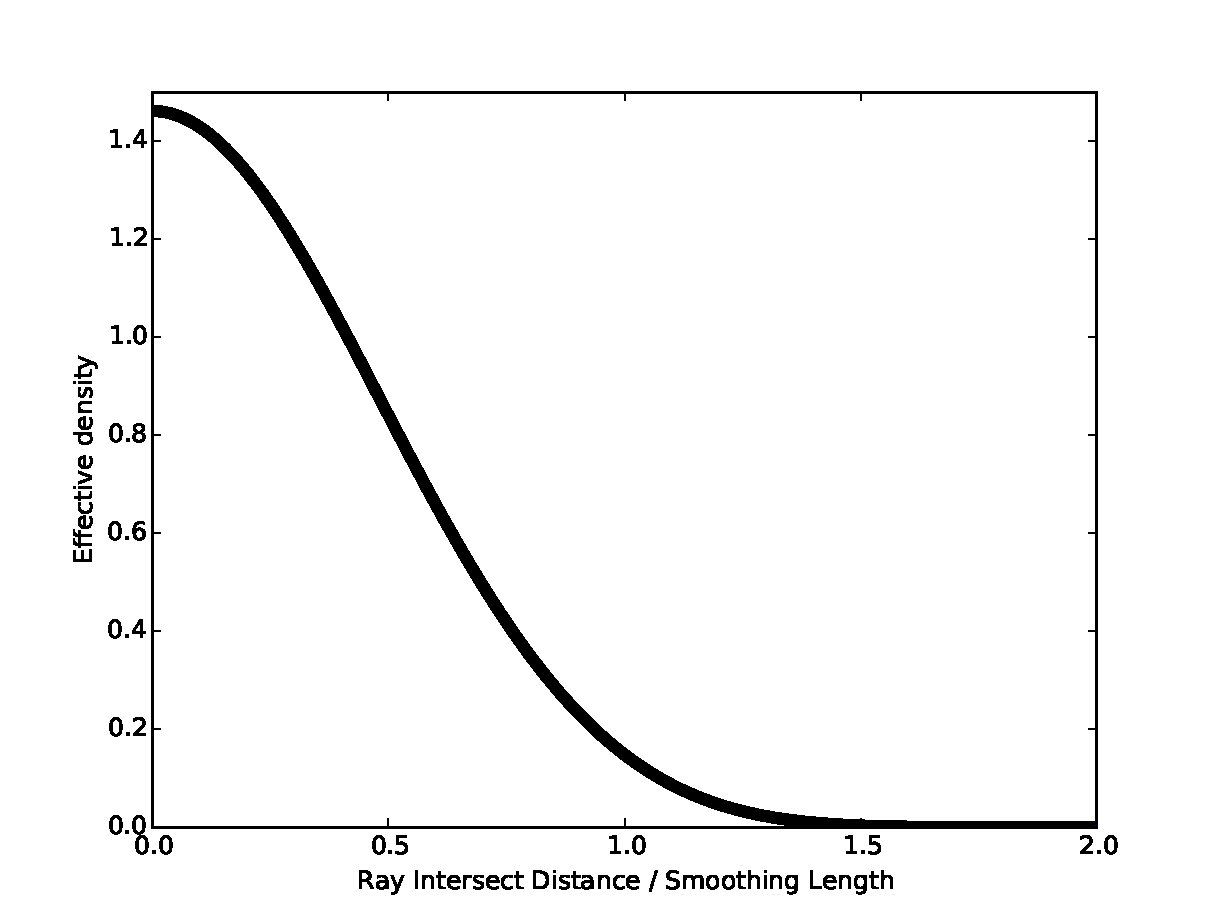
\includegraphics[width=0.85\textwidth]{plots/CH3/kernelPlot.pdf}
    \caption{Effective density of the M4 Cubic Spline smoothing kernel against radial distance from the particle}
    \label{smoothingKernel}
\end{figure}

While particle level tracing is only performed on particles within a chosen radius, in this case set as the SPH smoothing length of the source particle, efforts must be made to ensure that all particles who's smoothed mass fall within this radius are included. This may include particles in nearby cells that do not intersect with the ray even though some of their component particles do intersect due to the extra width generated by their smoothing lengths. For this, we initially refine all nodes within $h_{source} + h_{max, node}$ of the source, where $h_{max, node}$ is the maximum SPH smoothing length within the node. All particles within this distance are then sampled as normal.

Checks must be made to ensure that the particle does not contribute to its own optical depth as this can lead to substantially reduced flux values, particularly in matter with high optical depths. One other issue that must be prevented is where particles in close proximity all contribute each others optical depths due to overlapping smoothed mass regions, as shown in figure \ref{fig:ppOverlap}. This is the equivalent to two objects both being in front of each other simultaneously, a physical impossibility. To prevent this, all particles with a radial distance between themselves and the source greater than that of the sink particle being computed are ignored during the ray trace. This allows for optimization by ordering all particles in the node by ascending radial distance before performing the P-P calculation and ending the calculation at the first particle whose radial distance is too great. 

\begin{figure}[H]
    \centering
    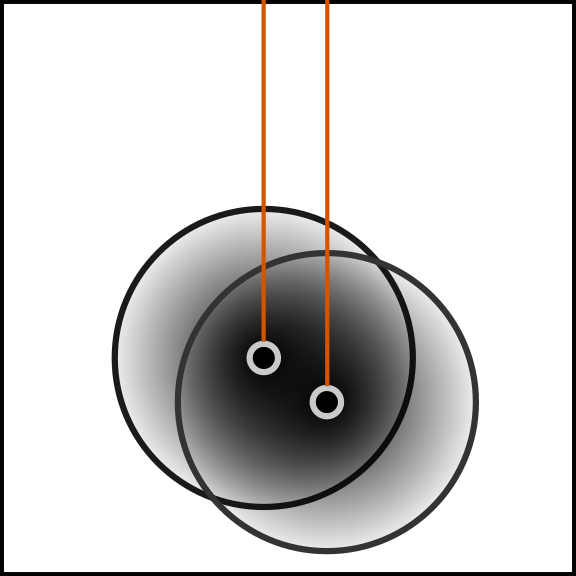
\includegraphics[width=\textwidth]{plots/CH3/ppOverlap.png}
    \caption{An example of two particles each contributing to the other's optical depth due their rays intersecting each others smoothed mass region.}
    \label{fig:ppOverlap}
\end{figure}
 % Implementation

%\lhead{\emph{Testing And Analysis}} 
\chapter{Testing and Analysis}

\section{The Optically Thin Case}

\subsection{Finding an Appropriate Opening Angle}
\label{sec:bangForBuck}
For this test we used a $64^3$ particle glass (see \citet{wadsley2017}) of source particles with an equivalent but rotated glass of sink particles to produce a well mixed system of sinks and sources. This was then perturbed using the sum of 24 sinusoidal modes, as shown in equation \ref{eqn:sinemodes},
\begin{equation}
    \label{eqn:sinemodes}
    \overrightarrow{r} = \overrightarrow{r_0} + \sum_{i=1}^{24} \frac{1}{275} \sin(k_{x,i}r_x + k_{y,i}r_y + k_{z,i}r_z + \phi_i).
\end{equation}
The wavevector components, $k_i$, are are in the range [-5, 5] and the $\phi_i$ terms are in the range [0, 2$\pi$] and assign random phases to each mode. The constant in front of the sine was selected to limit the amplitude of the density perturbations created by these modes to within reasonable bounds \citep{grond}.

The system was run with opening angles varying between 0.1 and 1 and the RMS error relative to an opening angle of 0 of each gas particle's flux was calculated. At the same time, the number of rays traced per sink was logged, giving us an indicator of the computational cost of each opening angle. Plots of both of these values against opening angle are shown in \ref{fig:openingTest}
\begin{figure} [H]
    \centering
    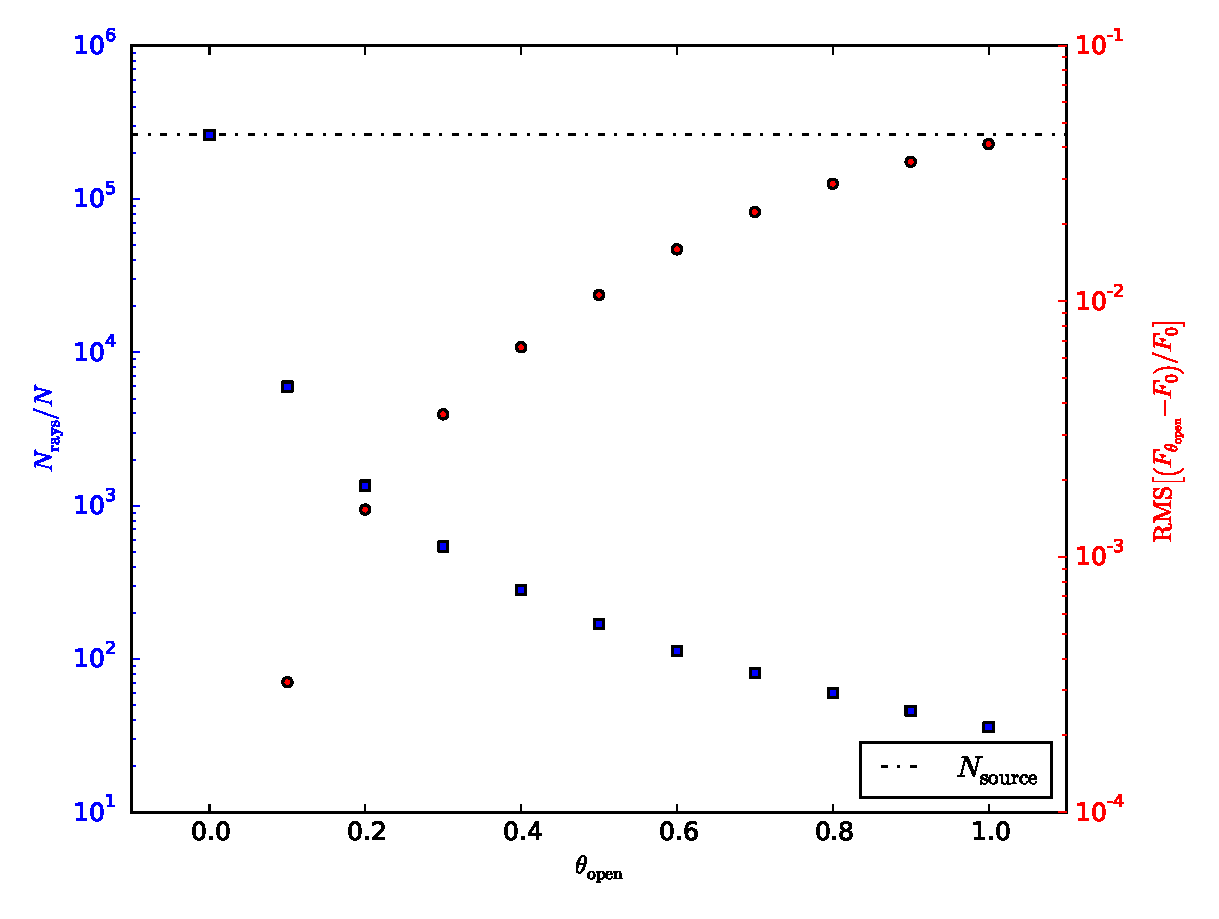
\includegraphics[width=\textwidth]{plots/CH4/opening_angle.pdf}
    \caption{RMS error and rays traced per sink for opening angles between 0 and 1.0}
    \label{fig:openingTest}
\end{figure}
After examining this plot, it was decided that we would use an opening angle of 0.5. This gives an RMS error of approximately $10^{-2}$ and a speedup of approximately $10^3$, i.e. requiring 0.1\% of the rays traced in the fully refined case. While this gives a good estimate of the appropriate opening angle for a well mixed system, simulations with dissimilar initial conditions may have differing optimal opening angles. These systems may benefit from repeating this test with ``toy" simulations that more closely approximate the system to find appropriate values for $\theta_{open}$. While testing the full simulation is possible, the time required to perform a full refinement test on a large system may make this challenging.

\subsection{Confirming Correct Scaling for Source Walk}

As the optically thin radiation algorithm is identical to that of gravity except for the force calculation, the scaling is identical at $\mathcal{O}(N_{sink} \log(N_{source}))$, as proven in \citet{grond}. To test this we used an identical initial condition to the previous test and changed the value of the opening angle from 0, giving full refinement, to an arbitrarily large value leading to no refinement. These are then compared to the minimum scaling of $\mathcal{O}(N_{sink} \log_2(N_{source}))$ and maximum scaling of $\mathcal{O}(N^2)$ in Figure \ref{fig:scalingThin}.

It can be seen that even a lower value of $\theta$ such as 0.4 still gives a substantial scaling improvement when compared to the full refinement, with ray counts up to nearly 3 orders of magnitude lower than that of the $\theta = 0$ test.
\begin{figure} [H]
    \centering
    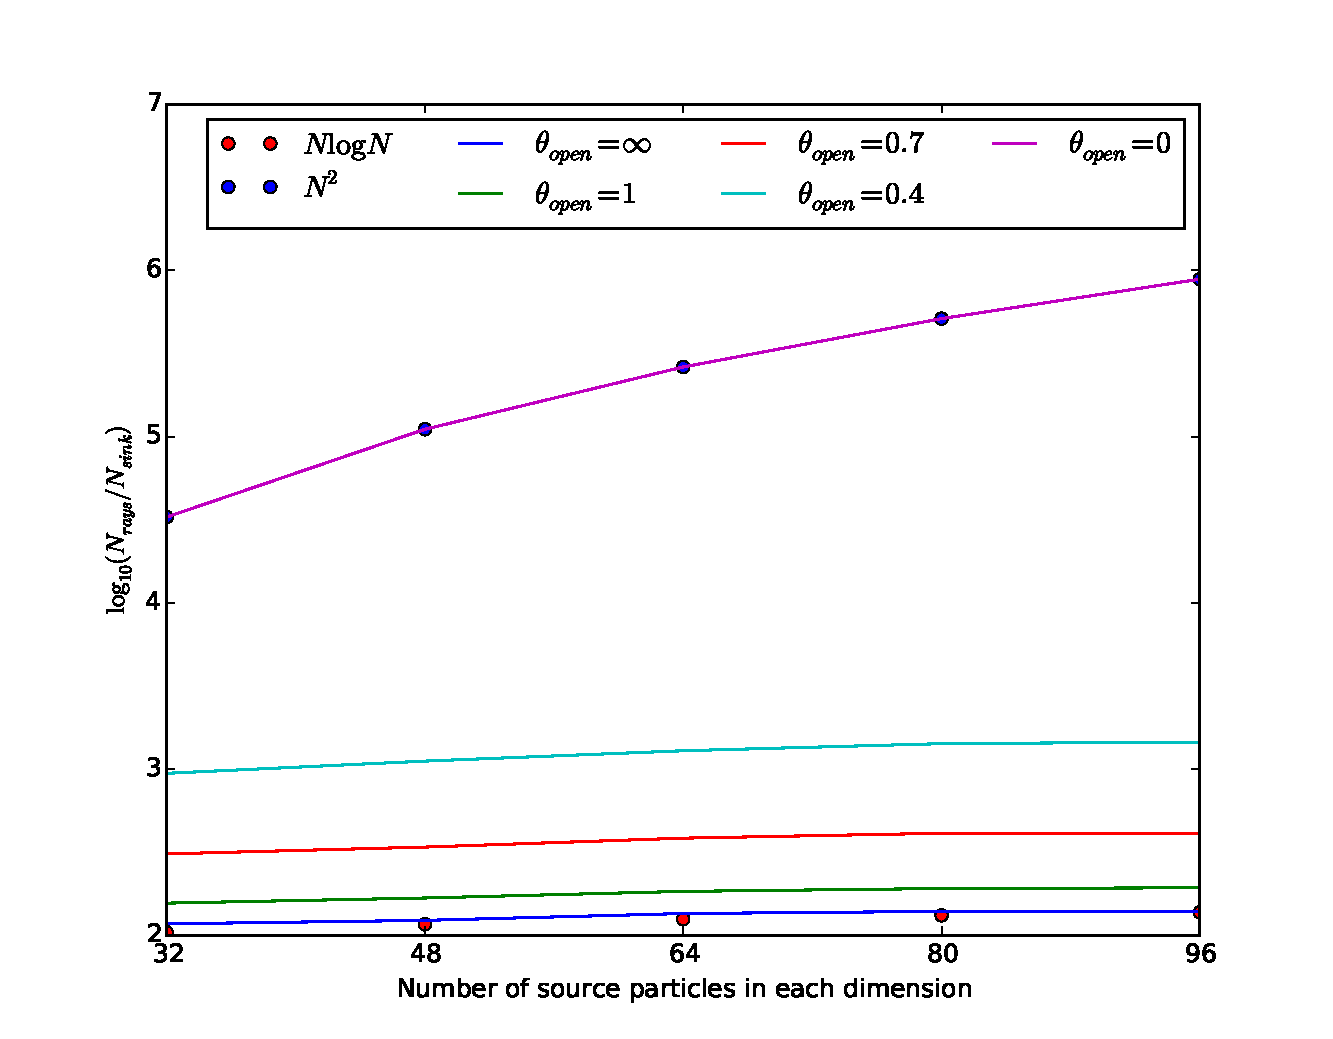
\includegraphics[width=\textwidth]{plots/CH4/scalingThin.pdf}
    \caption{Scaling of the optically thin (i.e. source walk) code. This is equivalent to that of the gravity walk}
    \label{fig:scalingThin}
\end{figure}
\subsection{Simulating Background Sources}

Some simulations require the creation of background sources to model such things as the cosmic ultraviolet background radiation. This can be approximated through the use of a sphere of background sources located at a great enough distance from the region of the simulation of interest with a luminosity that gives the required flux at the origin. This luminosity for each background source can be calculated by rearranging equation \ref{eqn:flux} in terms of L and dividing by the number of background particles, giving,

\begin{equation}
    L = \frac{4\pi r_{bg} F_{centre}}{N_{bg}},
\end{equation}

where $r_{bg}$, $F_{centre}$ and $N_{bg}$ are the radius of the background sphere, the expected flux in the centre of the system and the number of background particles respectively. 

Figure \ref{Fig:bgSource} shows the flux as a function of radius for a background source sphere at distance 0.5 from the simulation centre and an expected central flux of 1.0. It can be seen that the flux rapidly approaches the expected value of 1.0 with errors of only a few percent as far out as 0.2 from the centre. This implies that a reasonable proportion ($\sim 40 \%$) of the space contained by the background sources can be used for the simulation with minimal error in flux.

\begin{figure} [H]
    \centering
    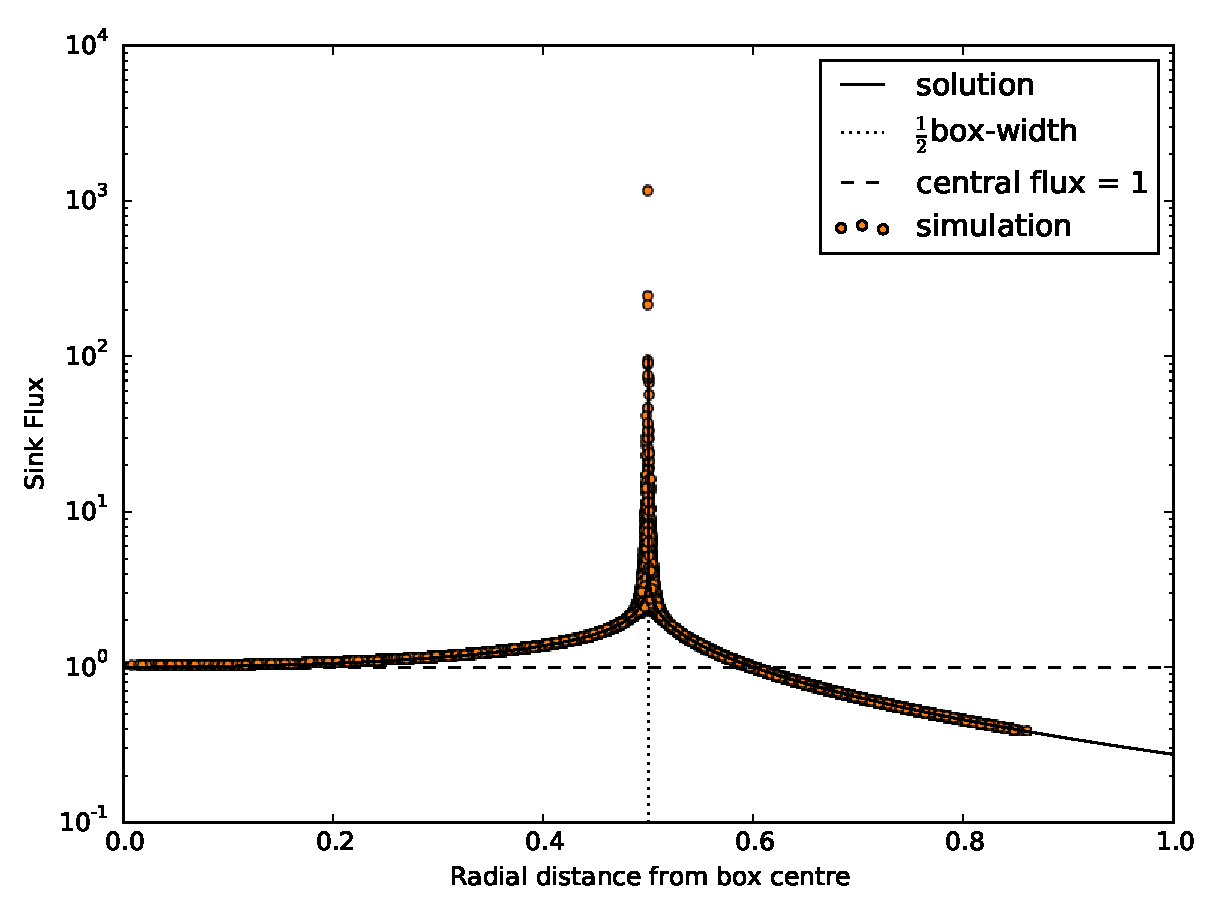
\includegraphics[width=0.7\textwidth]{plots/CH4/resultsCha.pdf}
    \caption{Flux against radial distance of background sources with total central flux of 1.0}
    \label{Fig:bgSource}
\end{figure}
    
\section{The Optically Thick Case}

\subsection{Uniform field test}
As an overall test of the accuracy of the optically thick code, we created a uniform gas field with 16 particles along each dimension whose optical depth across the box is 1, placed a star at the centre and measured the flux as a function of distance. As the absorption coefficient of this system is 1 in all space, the optical depth is exactly equal to the radial distance from the source, $r$. Thus, the simulated results can be compared to the analytical solution given in equation \ref{eqn:fluxUniform} to confirm that the optically thick code is functioning as expected,
\begin{equation}
    F = \frac{e^{-r}}{4\pi r^2}.
    \label{eqn:fluxUniform}
\end{equation}
Figure \ref{fig:uniformField} shows the results of this test, with the simulated results fitting near perfectly to the theoretical results.

\begin{figure} [H]
    \centering
    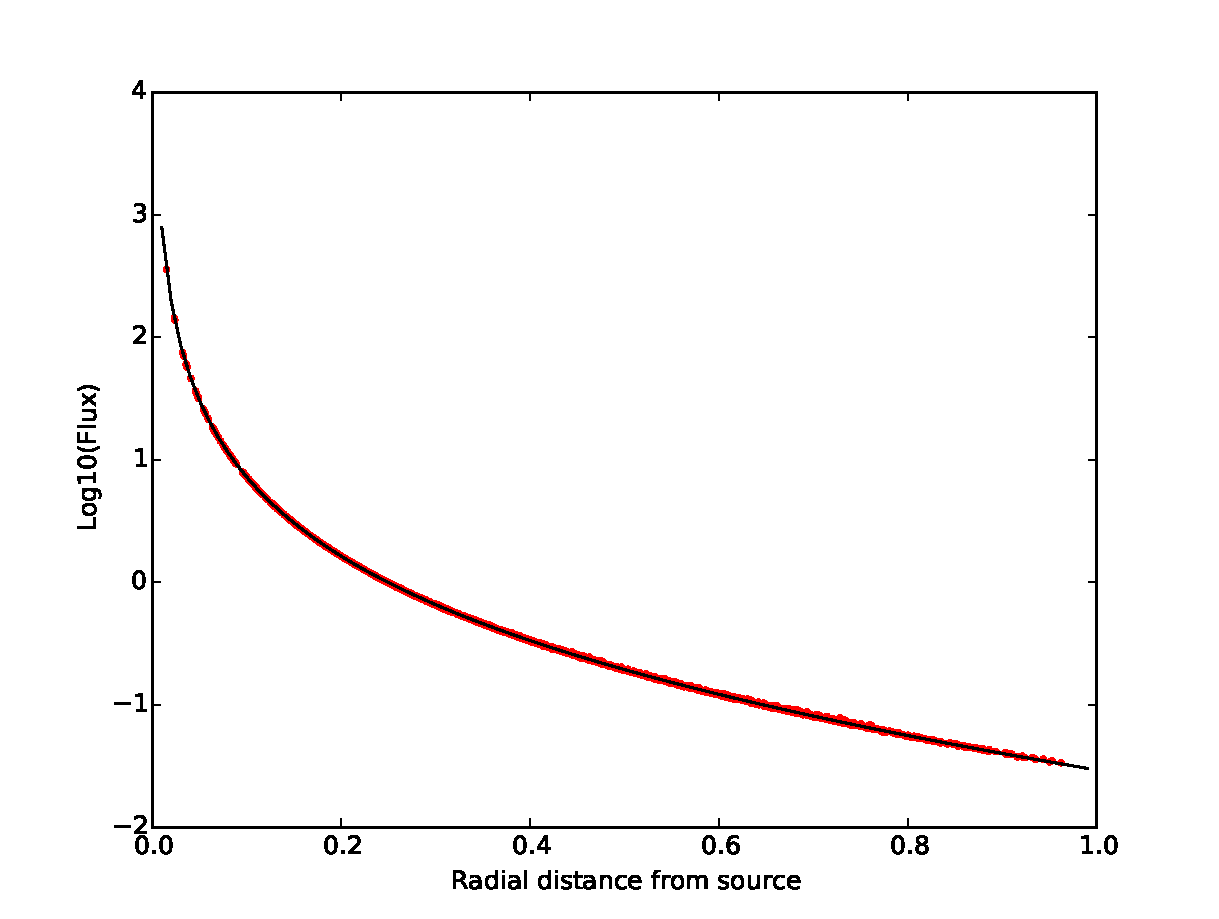
\includegraphics[width=\textwidth]{plots/CH4/thickFluxVr.pdf}
    \caption{Flux as a function of radius for a uniform density gas field compared to the analytic solution}
    \label{fig:uniformField}
\end{figure}

\subsection{Finding an Appropriate Maximum $\tau_{refine}$ Differential}

Finding an appropriate value for $\tau_{refine}$ can be done much the same way as finding the value for the opening angle, by changing its value and looking at both the speedup and the error. Unlike with the opening angle where we compared the number of rays, we instead compared the number of segments for all rays. 
\begin{figure} [H]
    \centering
    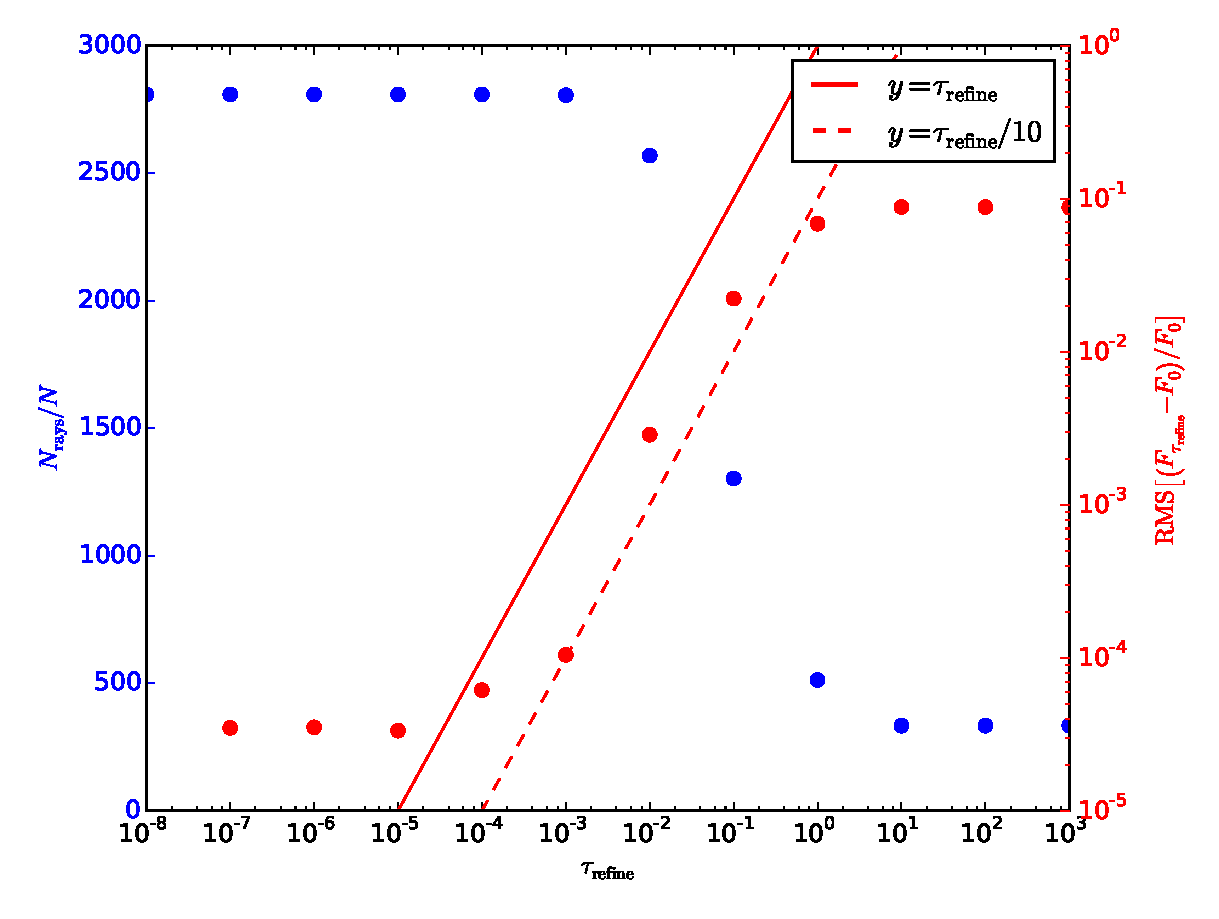
\includegraphics[width=\textwidth]{plots/CH4/tau_refine.pdf}
    \caption{Error in flux against maximum difference in $\tau$ of child nodes}
    \label{fig:maxTau}
\end{figure}
 The plateaus at both the lower and higher values of $\tau_{refine}$ are due to the limitations of refinement. For the lower values, this is caused by all values below $\tau_{refine} = 10^{-4}$ using purely bucket-scale absorption and for the higher values, only the P-P refinement criterion is being activated as the root node's $\tau$ perturbation is within permitted bounds. The two lines on Fig \ref{fig:maxTau} show the lines where the error is equivalent to $\tau_{refine}$ and $\tau_{refine}/10$. It can be seen that between refinement criterion values of $10^{-1}$ and $10^{-4}$, the error lies within these two lines, suggesting that the error in the absorption calculation is within an order of magnitude of the selected refinement criterion value. As there is no benefit to using a value of $\tau_{refine}$ lower than $10^{-3}$, optimal $\tau_{refine}$ was chosen to be between 0.1 and 0.01, depending on the accuracy required.

\subsection{Optically Thick Scaling Test}
To test the scaling of the Optically Thick code we once again ran simulations with increasing numbers of sinks and sources whose initial conditions are identical to that of the optically thin tests. The value of $\tau_{refine}$ was varied from 0.01 to an arbitrarily high value, i.e. no refinement, giving the results shown in Figure \ref{fig:scalingThick}. We chose 0.01 as the upper limit due to time constraints preventing us from running this test at full refinement.
\begin{figure} [H]
    \centering
    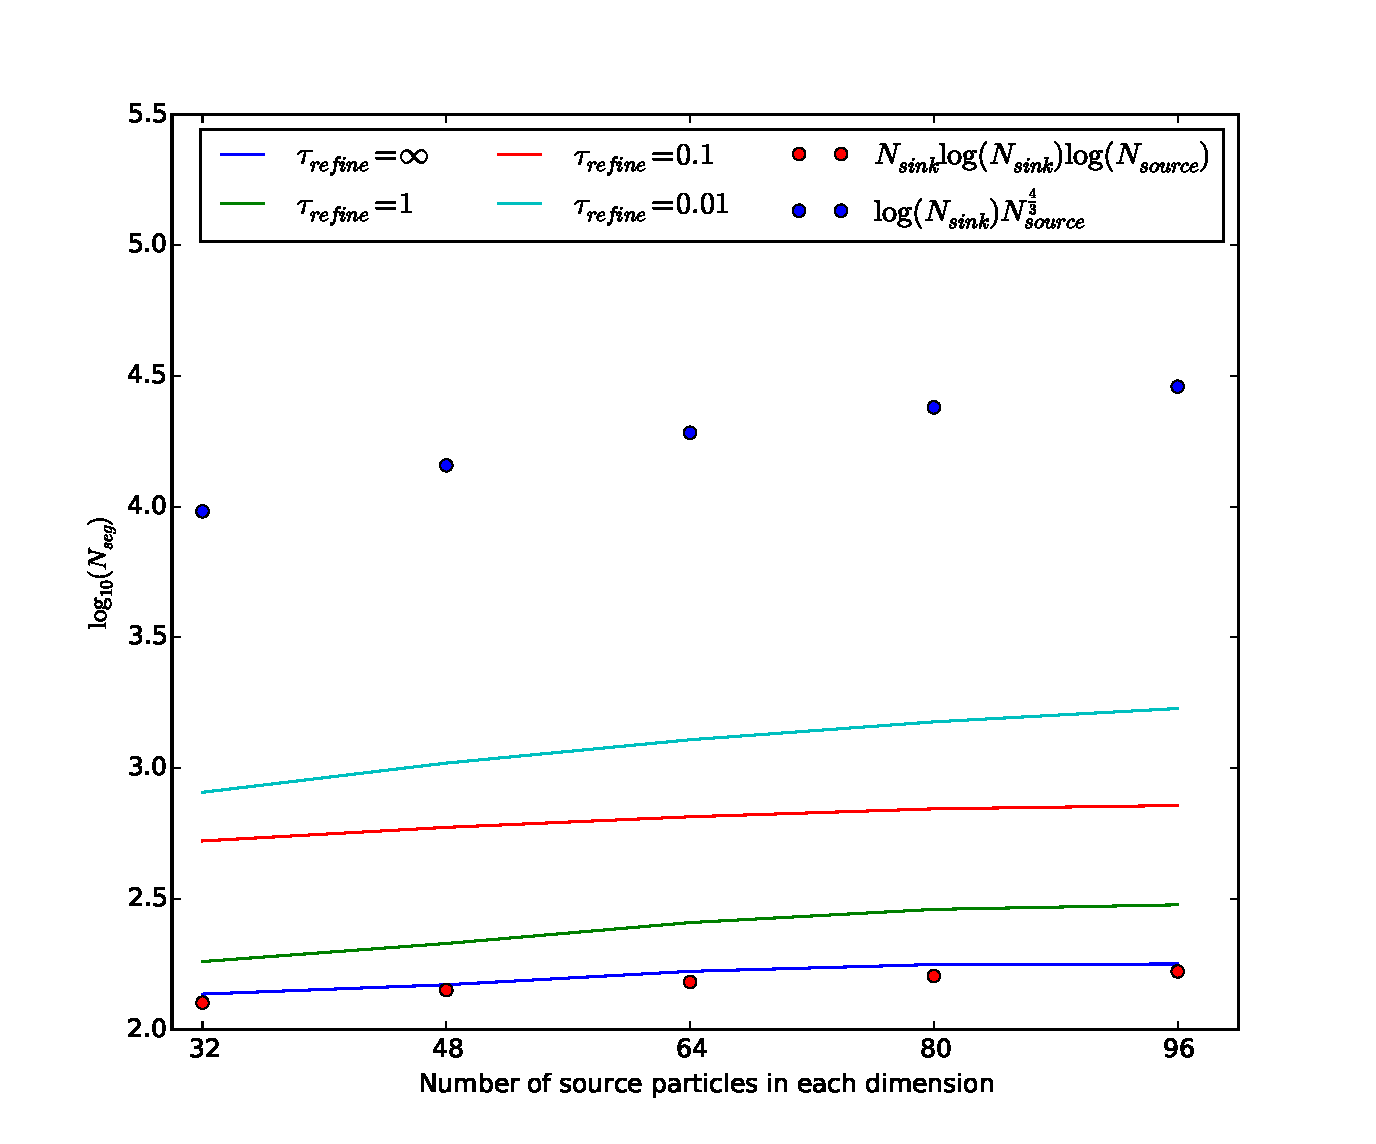
\includegraphics[width=\textwidth]{plots/CH4/tau_scaling.pdf}
    \caption{Scaling of the optically thick code.}
    \label{fig:scalingThick}
\end{figure}
The dotted values in Fig \ref{fig:scalingThick} show the minimum ($\mathcal{O}(N_{sink}\log{N_{sink}}\log{N_{source}})$) and maximum ($\mathcal{O}(N_{sink}^{\frac{4}{3}}\log{N_{source}})$) theoretical scaling. This maximum takes into account the reduction in computational cost from the source merging. Without this, the worst case scaling would be $\mathcal{O}(N_{source}N_{sink}^{\frac{4}{3}})$. It can be seen that the zero refinement case matches closely to the theoretical results and even lower values for the optically thick refinement parameter give strong scaling, with only a factor of 10 increase in the number of computations required.

\subsection{Isothermal Spheres test}

The isothermal spheres test was created to study the code's ability to create accurate shadows, regions where the flux from a source is blocked by dense objects. Multiple spheres whose densities follow a $\frac{1}{r}$ profile were created and placed with equal separation on the x = 0, z = 0 line. The source was placed at [-0.5, 0.4, 0], causing shadows behind the spheres with varying angular directions. 
\begin{figure} [H]
    \centering
    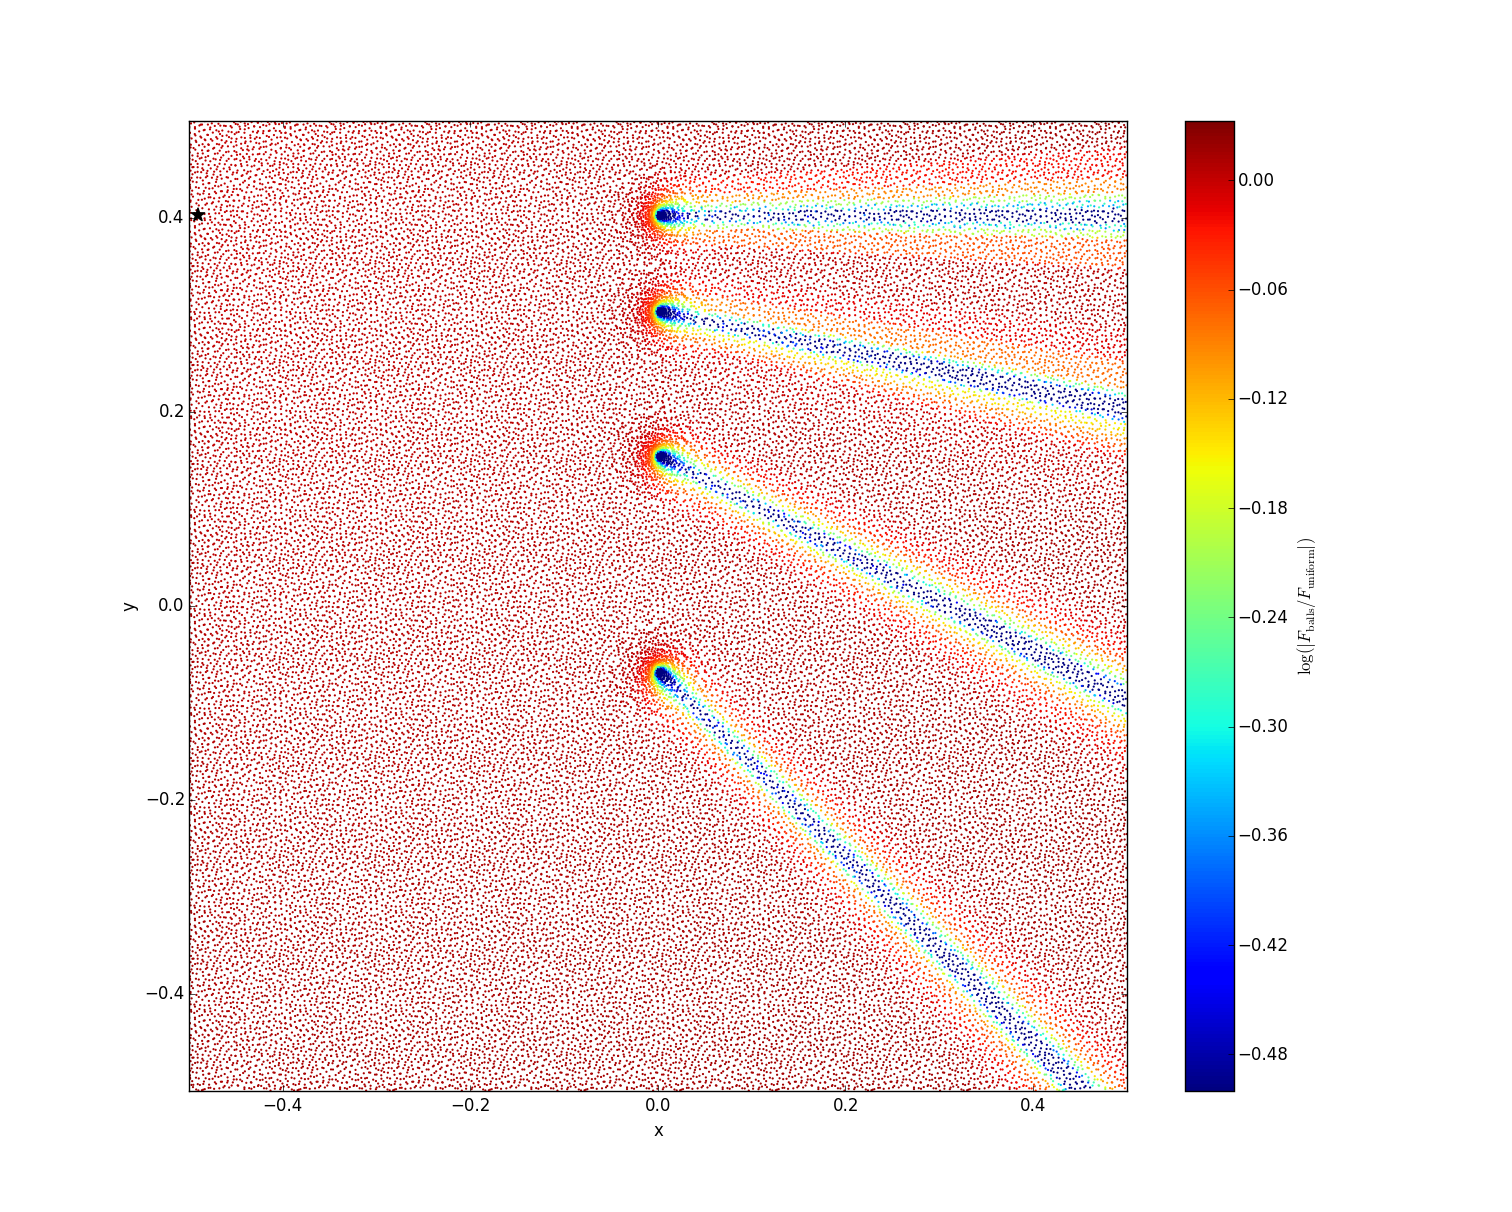
\includegraphics[width=\textwidth]{plots/CH4/balls_cha.png}
    \caption{Flux as a function of position of a uniform density gas with embedded isometric spheres. The data is normalized against the expected flux for an optical depth across the box of 1.0.}
    \label{fig:isoSpheres}
\end{figure}

The results for this test are comparable to those given in \citet{grond} where the errors are analyzed in detail.

\chapter{Complex sources}
\label{sec:complexsources}
The current refinement criterion for the source walk mimics that of gravity, where the only parameters that are used to determine whether a node should be opened or walked are the position and size of its bounding box. While this poses no issue when working with optically thin systems, when optically thick systems are treated the same way substantial error can arise. By moving the position of the sources in the node, we change the direction and dimensions of the ray walked between the sink and source and thus change the absorbing material intersected by the ray. Steps must be taken to make sure that any error introduced by source merging does not substantially alter the calculated flux and that the properties and distribution of the absorbing material are taken into account when selecting appropriate sources to perform ray tracing upon.

\section{Angular Dependence of Flux}
When sources are merged, the change in distance between each source and the sink at their initial, unmerged and their final, merged positions depend on the angle between the sink and source  node. This angle isn't taken into account when determining if a node should be opened and thus creates an error that is dependent on the angle on which the system is observed. For the optically thin case, these errors are second order and oscillate around zero with only a weak systematic bias. For randomly oriented source pairs there would be no systematic bias.

This can be shown by studying a system with two sources embedded inside a dense sphere, with each source an equal distance from the spheres centre. By taking measurements of the flux from both the combined and uncombined sources along a circle centred on the sphere and with a radius larger than the sphere radius we can see the error created by source merging. Figure \ref{fig:CSIC} shows the setup used to test this issue, with a sphere of radius 2, selected to represent a distance where source merging would occur, and sources embedded at a distance of 0.5 along the x-axis, either side of the sphere's centre. 
\begin{figure} [H]
    \centering
    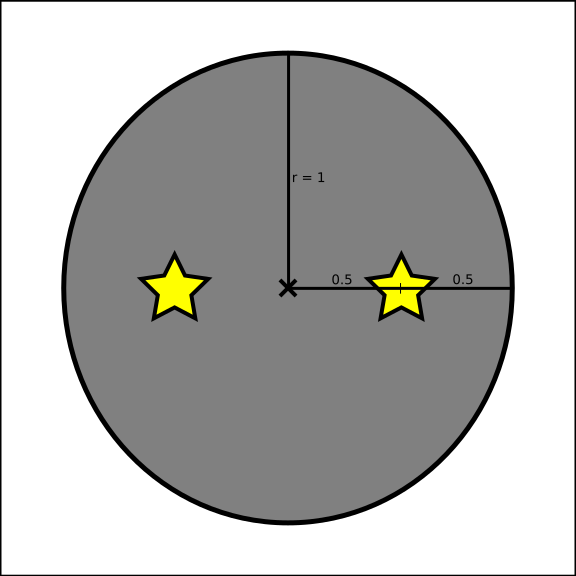
\includegraphics[width=\textwidth]{plots/CH4/CSICs.png}
    \caption{System setup for the angular dependence test}
    \label{fig:CSIC}
\end{figure}
The optical depth along the radius of the sphere was varied from 0 to 16, giving the error of the merged sources as a function of angle, shown in figure \ref{fig:CSAngular}.

\begin{figure} [H]
    \centering
    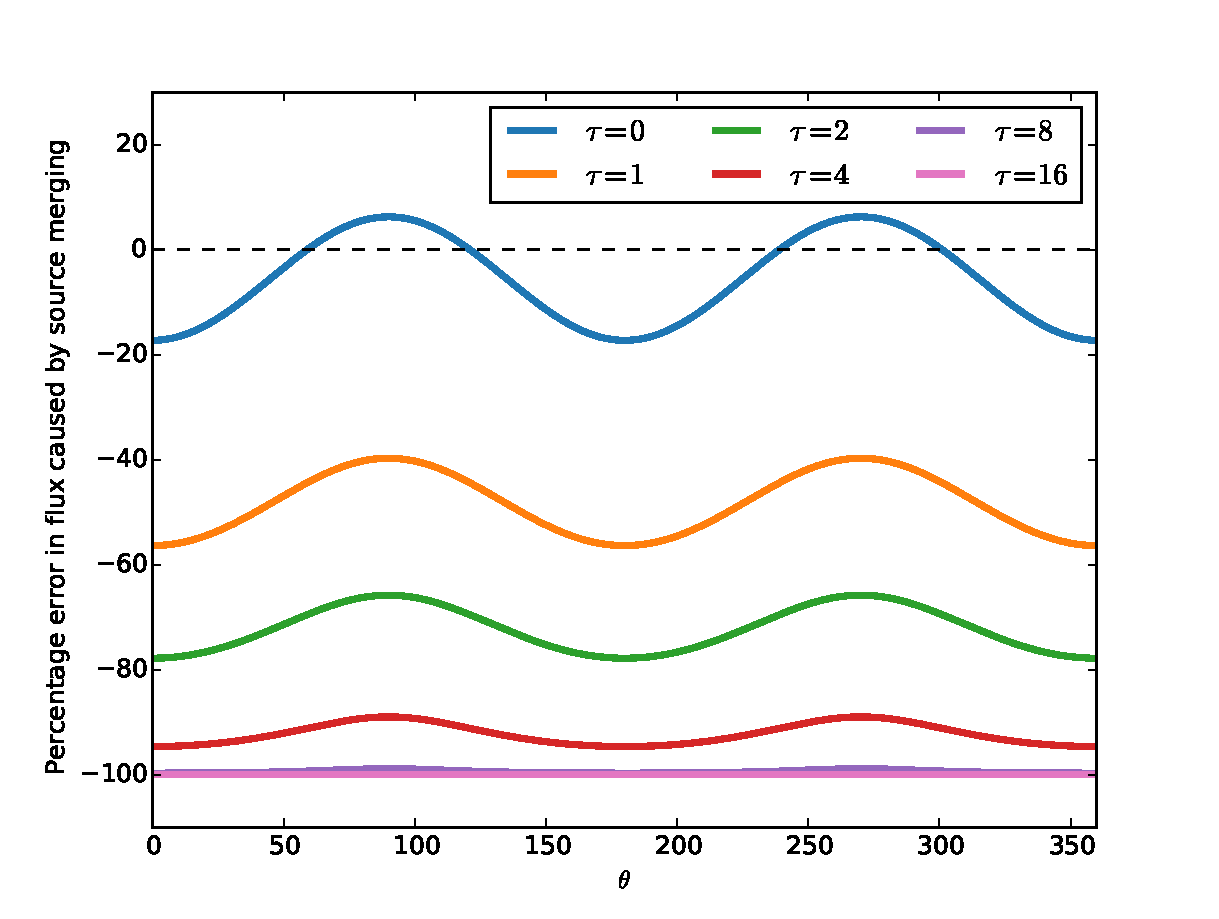
\includegraphics[width=\textwidth]{plots/CH4/CSError.pdf}
    \caption{Percentage error in flux due to source merging as a function of flux for varying optical depths}
    \label{fig:CSAngular}
\end{figure}

While the initial conditions used are simple, the systematic trend towards lower values for the flux when merging is what is expected in typical astrophysical set-ups where sources are embedded in absorbing material, this this suggests that this gives a reasonable toy model of real scenarios. Only scenarios such as sources merging into a region with a noticeably lower optical depth would cause systematic positive errors in the flux. This could occur but is less likely so we speculate that systematic reductions in flux are the most likely outcome.

The error in the flux caps at 100\% (i.e. $\sim$ 0 flux is received) at $\tau = 16$, with the plot suggesting that the error increases dramatically as one moves to higher optical depths. However, only looking at the percentage error doesn't take into account the absolute flux received by the sinks, shown in figure \ref{fig:CSAbsError}.

\begin{figure} [H]
    \centering
    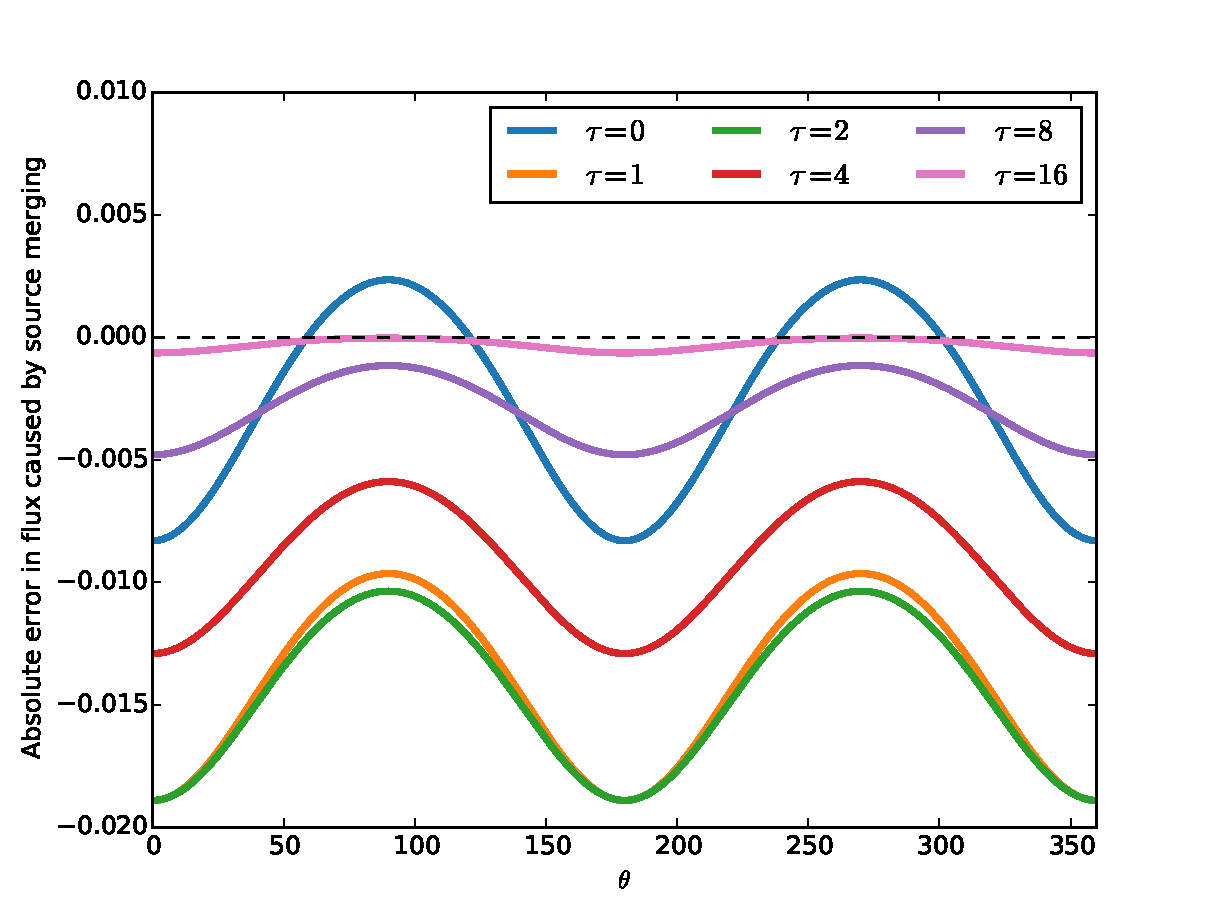
\includegraphics[width=\textwidth]{plots/CH4/CSAbsError.pdf}
    \caption{Absolute error in flux due to source merging as a function of flux for varying optical depths}
    \label{fig:CSAbsError}
\end{figure}

Of note is how the absolute error in the system peaks at approximately $\tau = 2$ before returning to approximately 0 at extreme values of $\tau$. This is due to the increase in optical depth reducing the magnitude of the flux able to escape the dense region resulting in a low absolute error regardless of the high percentage error. This suggests that regions with intermediate optical depths (order 1-2) suffer from the greatest error. Unfortunately, a large proportion of astrophysical systems fit into this category and thus makes solving the complex sources problem one of importance for accurately modelling radiation in astrophysical radiative transfer simulations.

\section{Resolving Complex Sources}

\subsection{Utilizing an Optical Depth Refinement Criterion}

The simplest approach is to implement a modification of the refinement criterion from the optically thick walk in the source walk. This would allow the source refinement to take into account the absorption properties of each node and only require minimal coding. Instead of looking at the optical depth differential, we instead take the distance that the child sources must move when merging and multiply it by the absorption coefficient for the node, giving the optical depth from source merging. If this optical depth is greater than a chosen refinement value, we refine on that node and all descendant nodes.
\iffalse
This was implemented into the tree build and ran on identical initial conditions to the opening angle tests shown in figure \ref{fig:openingTest}. A plot of the number of nodes flagged for refinement as a function of $\tau_{refine}$ is shown in fig \ref{fig:CSnumNodes}. The number of nodes flagged is comparable to the number of sources used and thus gives us an estimate of the cost.

\begin{figure} [H]
    \centering
    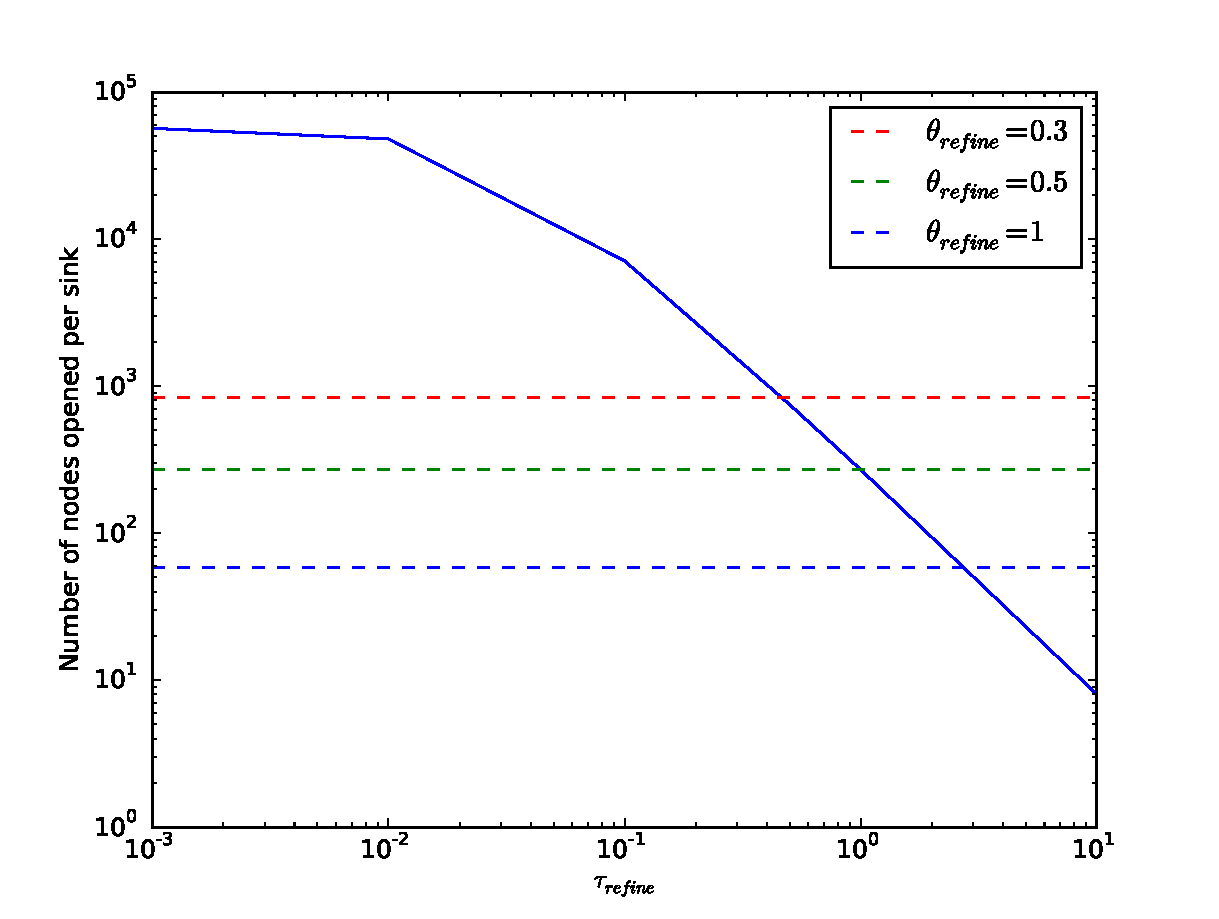
\includegraphics[width=\textwidth]{plots/CH4/CSOpeningTau.pdf}
    \caption{Number of tree nodes marked for refinement as a function of maximum perturbation in $\tau$ through a node with node opening counts of tree walks for $\theta_{refine}$ values of 0.3, 0.5 and 1 for comparison}
    \label{fig:CSnumNodes}
\end{figure}

It can be seen that utilizing a value for $\tau_{refine}$ similar to that used in the optically thick tree walk will result in substantially more nodes being opened, with approximately 2 orders of magnitude between our standard $\theta_{refine}$ value of 0.5 with no complex source refinement and the same with our standard $\tau_{refine}$ value of 0.01 used for complex source refinement.
\fi
As this method is only sensitive to the perturbation in the optical depth, it is of little use in scenarios such as those shown in figure \ref{fig:CSIC} where the density across the node is constant. As figures \ref{fig:CSAngular} and \ref{fig:CSAbsError} show, even constant density regions can cause large errors in the flux when merged. On the other hand, this method is excellent at finding cases where variations in the optical depth can cause the merged sources to drastically change the optical depth of the regions traced by the ray. This, combined with the method's low computational cost, suggests that this refinement criterion would work best when combined with others with each criterion working to eliminate a specific sub-type of complex source.

\subsection{Ray Tracing During Tree Build}

A more involved method for resolving the complex source problem is to utilize a simplified optically thick ray trace during the tree build that compares the variation in flux of combined (parent) and uncombined (child) sources to a sphere of background absorbers centred on the node, as shown in fig \ref{fig:CSrefExample}. The radius of this sphere should be set as equal to or greater than the distance that the node's sources would merge, calculated via equation \ref{eqn:openingTheta}. If the angular variation of the error in the calculated optical depths is too great, a variable in the parent node that tracks if precalculated refinement is necessary can be set to true. All nodes with this node as a descendant are also set to open without tracing. This results in every node refining to the first combined source that is deemed an accurate representation of their child nodes.

\begin{figure} [H]
    \centering
    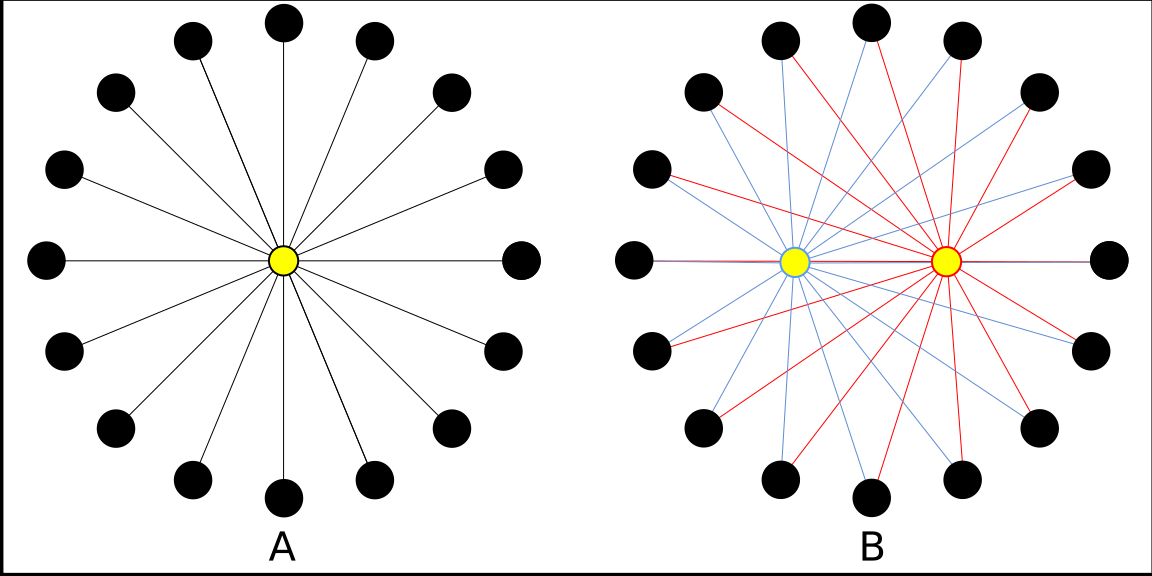
\includegraphics[width=\textwidth]{plots/CH4/CSDiagram.png}
    \caption{Diagram of the ray traces performed on parent (A) and child (B) nodes for the complex source refinement test during the tree walk}
    \label{fig:CSrefExample}
\end{figure}

Once this computation has been performed the refinement test during the tree walk can again be completed with minimal computational cost, only requiring a check to see if the node is flagged for refinement.

As each node will only have its centre of luminosity traced to a predetermined number of fake sinks, this method has a cost of only $\mathcal{O}(N)$ (where N is the number of nodes, which is proportional to the number of particles) but risks creating a scenario in which the reduction of computational cost given by the source walk opening criterion is nullified by the forced opening when complex sources are detected. 

This method can also be utilized for another purpose: direct flux correction. As figure \ref{fig:CSAbsError} clearly shows, there is a strong negative bias in the calculated flux when merging sources even for the optically thin case. By taking measurements of the error in the optically thin flux across the full sphere of the sky around the node, we can calculate an average flux bias and modify the absorption properties of each ray trace to mitigate this. This can be done by storing a correction factor that can be applied to each ray's calculated optical depth to account for the average flux loss due to source merging. Alternatively, a collection of values from a range of directions could be stored and the correction factor extrapolated from the combination of these values and the direction of the ray, although this would require more extensive data storage.

\subsection{Flux Tracking}

One method that can be used to reduce the cost of an increased sensitivity refinement criterion is flux tracking. This is where the total flux received by a sink is retained to the next timestep, allowing an estimate of the flux from each source to be calculated. If a source is estimated to contribute only a minor amount to the total flux, there is minimal benefit to fully resolving any complex sources. This relates to the fact, as shown in figure \ref{fig:CSAbsError} that the absolute error can be quite small for deeply embedded sources This allows for the added computational cost to be focused primarily on the sources with the greatest impact on the flux which keeps the total error bounded.

An alternative method is to use the optically thin flux of the sources from the current timestep and apply a optical depth estimator where the ray length is the euclidean distance between sink and source and the absorption coefficient is the averaged value for the entire box. All sources are found before commencing ray tracing and thus the total flux estimate can be calculated prior to the ray trace walk. The estimated contribution from each ray can then be compared to the total flux. This method can be combined with the optically thick refinement to help minimize its cost, although this would limit its ability to pre-calculate the refinement outcome during the tree build.

Care must be taken when applying this criterion due to the systematic negative error in the flux caused by merging. Any node that is merged will contribute to this error and thus applying this criterion without taking this into account will almost always increase this systematic error. Estimating a correction factor based on the the faction of the prior flux that the merged sources contributed could reduce this error but this risks forcing the total flux to remain at a constant value. Another option is to base the factor on the optically thin flux contribution estimate.

It should be noted that flux tracking can identify sources that are negligible regardless of complicating factors and which thus can be terminated. This technique could be applied to neglect even simple sources and save work. The challenge is to use a sufficiently conservative estimator to ensure the sources designated to be neglected are guaranteed to be small contributors. If the total flux is the product of many weak sources, then none of them can be neglected otherwise a systematic error is created. In addition, selecting a cruder representation (e.g. source merging) also requires care if the flux errors are systematic.
    
 % Testing

%\lhead{\emph{Conclusion and Future Research}}
\chapter{Conclusion and Future Development}

\section{Conclusion}

In this thesis we discussed radiative transfer in astrophysics, listing the common algorithmic methods for application in astrophysical simulations. We presented an overview of reverse ray tracing, its benefits and limitations compared to forward ray tracing as well as the existing codes that employ it before giving a summary of the TREVR radiative transfer method. We gave details of the GASOLINE astrophysical simulation code as well as the use of trees for source merging. Reverse ray tracing is an area of active interest in the astrophysical simulation community but techniques are still being developed and code papers to date tend to be incomplete, with few tests that fully study their accuracy and scaling. Much of reverse ray tracing was developed for post processing, where crude accuracy was acceptable or one could change parameters until desired results were achieved. Now that it is being simulated during run time, often with the output directly linked to other systems such as cooling, this lack of accuracy has become an issue. In particular, we identified an issue with complex sources that no previous code has addressed. This was detailed in Chapter \ref{sec:complexsources}.

We presented the ChaNGa radiative transfer code and the Charm++ framework that it utilized, comparing it directly to GASOLINE, particularly in areas such as the combined tree build and top down tree walk. We described the core components of the Charm++ framework that allowed for us to simplify the development process, such as Chare and Message objects. As part of this development we realized that for all the appeal of the Charm++ framework, the final products, e.g. ChaNGa, are unwieldy and more challenging to develop compared to other codes such as GASOLINE. We strongly advocate that ChaNGa needs to be refactored to improve usability, saving substantial work for future developers. We note that this has already been done for SPH in ChaNGa, resulting in a clean implementation that is likely better than the GASOLINE implementation to work on.

We discussed the development process for both the optically thin and optically thick walks, the methods for calculating the flux and optical depth of the ray, as well as their refinement criterion $\theta_{open}$ and $\tau_{refine}$. We also discuss particle level refinement and how the utilization of a SPH-like method is necessary to accurately calculate the flux when interacting with individual particles. Using our experience with GASOLINE we were able to develop simpler and more efficient algorithms for the ChaNGa implementation. These tests confirm the useful scaling of the TREVR method now implemented in Charm++.

We tested the code so developed by comparing the simulation results with analytical models for simple systems as well as the isothermal spheres test developed and described in detail in \citet{grond}. In particular, we note that the tests in  Grond et. al. are far better than those typically presented in other recent radiation code papers. In particular, error estimates are typically unavailable for many methods. We tested multiple values of $\theta_{open}$ and $\tau_{refine}$, studying the error for each value. Due to the quantitative tests developed by Grond et. al. we were able to suggest optimal values. We also recorded the number of rays or ray segments traced during the tree walks, using this as an analogue for the computational cost of the system and allowing us to see the cost increase for each refinement value and thus compare the cost to the error for each refinement value. It would be good to firmly establish the value of ray segments as a good proxy for actual work (e.g. wall clock time). We note that the ChaNGa implementation still has rough edges and some parts need to be optimized before such testing would be relevant.

Finally, we discussed the Complex Sources problem, where the merging of sources can cause systematic errors in the calculated flux for optically thick problems while also creating an angular dependence on its accuracy. We showed that merging nearly always causes a negative error in the flux received by a sink regardless of the optical depth of the system, and that the errors peaked for intermediate values of $\tau$. Such scenarios are common in astrophysical simulations. We propose several methods for the mitigation of this issue such as the application of a modified form of an optically thick refinement criterion on the source finding walk and ray tracing to a limited number of sources and studying the angular variation in optical depth. Both of these methods can be run during the tree build, allowing for the refinement to be checked once for all particles. We anticipate that this will suffer from the issue of over-refinement, dramatically increasing the computational cost of the radiative transfer code and offer a method for limiting this in the form of flux tracking. 

\section {Future Development}

Below is a selection of future additions to the ChaNGa radiation code that we were unable to implement due to time constraints or what fell outside the focus of this thesis.

\subsection{Volumetric Rays}

Infinitesimally thin rays, or ``pencil beams" that are used in many ray tracing methods including our own are computationally simple, only requiring a length to be calculated to give each segment's optical depth contribution. As shown in the discussion of complex sources, small changes in the path of the ray being traced can result in substantial changes in the calculated optical depth. Pencil beams suffer a similar issue where sources have a portion of their solid angle in the sky obscured by absorbers but whose centre of luminosity remains unobscured would give incorrect values for their flux compared to a fully refined computation. Unlike with the complex sources problem, this issue is due to the change in absorbers intersected by the ray rather than the interaction of sources and absorbers during the tree build.

A method of resolving this issue is to use non-pencil or ``volumetric" beams similar to those implemented in \citet{treeRay}. Each node's bounding box would interact with a section of the volume of the ray rather than a simple line segment, with equivalent for the particle level refinement. The flux from the source would be distributed across the volume in a similar method to the mass distribution of an SPH particle, with the majority of the flux contained within the centre. Calculating each node's contribution to absorption would require the beam to be integrated with bounds given by the node's bounding box limits. This would require substantially more computation than the pencil beam method and due to the increased volume contained within the beam, many more nodes would be intersected. 

It should be noted that for volumetric rays the correct method to average absorption is less clear as compact, dense objects will quite often only partially block a volumetric ray, regardless of how optically thick the object itself is. This issue was not fully addressed by Haid et al.

\subsection{Combined Particle Ray Trace}

Currently, the particle level contribution for the optical depth is computed for all sink particles individually and run during the tree walk for each sink. This results in the need to refine to the bucket level for all nodes within the P-P radius of all sinks, substantially adding to the computational cost of the system.

An alternative method would be to create a list of absorbers that require particle level refinement for all sinks in the bucket at once, using a P-P refinement radius equal to the value of d where,
\begin{equation}
    d = r_{COL}+h_{SPH},
\end{equation}
with $r_{COL}$ and $h_{SPH}$ referring to the sink-centre of bucket distance and the smoothing length of each particle respectively. The list created would contain absorbers that may not apply to some particles but once the costly particle collection step has been performed, the list of absorbers can be filtered for each sink with minimal cost. This would mean that during the tree walk, nodes within the P-P radius would not require full refinement, only refinement until some of their sibling nodes do not intersect the radius. The non-PP contribution can then be calculated as normal and the walk continued.

\subsection{Multiple Radiation Bands}

The code is currently written to only allow for tracing of one radiation band at any time. This reduces its utility in systems that are optically thick to certain wavelengths but thin to others of interest. Much of the existing code could be easily extended to utilize vector-based radiation properties, including during the tree build. Each node would require a band-specific absorption coefficient along with band specific luminosities and centres of luminosity and each particle would likewise require band-specific values for their radiation properties.

The code for the tree walk and tree build could be left much the same, only requiring additional code to act on all bands instead of one. The optically thick refinement criterion would become more complex as multiple bands would give varying results. The safest choice would be to refine whenever any band requires it as the actual optical depth summation work is small.

\subsection{Source List Hash Table}

Currently, the way that particle and node data are stored for the optically thick tree walk results in data duplication, with sinks which each have the same source both storing all of the source's properties. A far more efficient method would be to replace this with a hash table system, where the source properties are stored in a hash table and only the table key is recorded in the source list. This would greatly reduce data usage in systems with a large number of sources or where the refinement criterion for source merging is particularly stringent while having little impact on the computational cost of the code.

Another benefit of this method is that with a full list of sources and sinks, the full system can be walked at once, creating something similar to the full sky column density maps seen in \citet{treeRay}. This would have a scaling of $\mathcal{O}(N_{sink}\log(N)$ when traced out from the sink, substantially reducing the computational cost of the system. % Future

%\input{Chapters/Chapter6} % Results and Discussion

%\input{Chapters/Chapter7} % Conclusion

%% ----------------------------------------------------------------
% Now begin the Appendices, including them as separate files

%\addtocontents{toc}{\vspace{2em}} % Add a gap in the Contents, for aesthetics

%\appendix % Cue to tell LaTeX that the following 'chapters' are Appendices

%\chapter{An Appendix}
	% Appendix Title

%\input{Appendices/AppendixB} % Appendix Title

%\input{Appendices/AppendixC} % Appendix Title

\addtocontents{toc}{\vspace{2em}}  % Add a gap in the Contents, for aesthetics
\backmatter

%% ----------------------------------------------------------------
\label{Bibliography}
\lhead{\emph{Bibliography}}  % Change the left side page header to "Bibliography"
\bibliographystyle{unsrtnat}  % Use the "unsrtnat" BibTeX style for formatting the Bibliography
\bibliography{Bibliography}  % The references (bibliography) information are stored in the file named "Bibliography.bib"

\end{document}  % The End
%% ----------------------------------------------------------------